\pdfbookmark{Общая характеристика работы}{characteristic}
\section*{Общая характеристика работы}

\pdfbookmark[1]{Актуальность}{actuality}
\underline{\textbf{Актуальность темы.}}
Искусственный интеллект (ИИ) активно развивается и успешно применяется в робототехнических задачах, где роботу необходимо принимать решения в каждый момент времени. Обычно такое обучение проводится на заранее собранных данных или в симуляторах. Однако важным свойством общего искусственного интеллекта является способность к адаптивному дообучению в реальных условиях, которые могли быть не учтены при обучении.

Методы обучения с подкреплением (Reinforcement Learning, RL) имеют большой потенциал для дообучения робототехнических систем в реальных условиях. В таких методах агент обучается методом проб и ошибок: он получает вознаграждение за действия, приводящие к желаемому поведению, а само вознаграждение используется как численный сигнал, описывающий цель обучения. Одним из важных навыков, приобретаемых агентом в процессе обучения, является исследование среды для поиска более эффективной последовательности действий при решении исходной задачи. Однако в реальных условиях действия робота во время исследования могут нанести вред людям, окружающей среде или самой робототехнической системе. Поэтому агент должен исследовать среду безопасно; эту задачу рассматривает область безопасного обучения с подкреплением (Safe Reinforcement Learning, Safe RL).

По аналогии с вознаграждением в безопасном обучении с подкреплением вводится штраф, численно описывающий ограничения, которые робот должен соблюдать. Одна из ключевых проблем этой области состоит в необходимости решать двойственную задачу: с одной стороны, агент должен научиться выполнять поставленную задачу, например достигать цели; с другой стороны, он должен соблюдать требования безопасности, например не превышать скорость, не приближаться слишком близко к препятствиям или снижать скорость рядом с людьми. Оптимизация таких ограничений часто приводит к тому, что робот предпочитает оставаться на месте и не решать исходную задачу, чтобы не нарушать ограничения.

Одним из классических семейств подходов к решению этой задачи являются лагранжевы методы, решающие двойственную задачу Лагранжа. Такие методы обычно применимы к произвольной среде, однако не обеспечивают строгих гарантий безопасности. Другое семейство методов предполагает априорное знание о среде, например использование барьерных функций. В этом случае требуется знание модели объекта управления, явного вида функции штрафов и её дифференцируемости. Хотя такие методы могут обеспечивать требуемый уровень безопасности, они часто требуют большого числа взаимодействий со средой, что трудно реализовать на реальной робототехнической системе.

Обучение с подкреплением на основе моделей мира позволяет частично решить эту проблему. В таком подходе, помимо стратегии агента, обучается модель мира, позволяющая заранее предсказывать будущие состояния среды при выполнении заданных действий. Модели мира позволяют, во-первых, генерировать дополнительный синтетический опыт и тем самым уменьшать число взаимодействий робототехнической системы со средой, а во-вторых, заранее оценивать, приведёт ли последовательность действий к нарушению требований безопасности.

Методы безопасного обучения с подкреплением на основе модели мира позволяют повысить безопасность агента при меньшем количестве взаимодействий со средой, что является важным условием применения таких методов на робототехнических установках. В этих подходах безопасное исследование зависит от того, насколько корректно модель мира оценивает будущую стоимость действий. Если риск недооценён, агент может выбирать небезопасные траектории; если риск переоценён, агент становится чрезмерно консервативным и прекращает активное исследование среды. Поэтому качество оценки долгосрочной стоимости является ключевым фактором для баланса между достижением цели и соблюдением ограничений безопасности. Тем не менее методы безопасного обучения с подкреплением на основе моделей мира также сталкиваются с ограничениями в задачах с большим горизонтом. Такие задачи обычно характеризуются одним или несколькими факторами: большим числом действий, необходимых для достижения цели; разреженной функцией вознаграждения, при которой агент редко получает обучающий сигнал; высокой размерностью пространства состояний и действий.

Одним из направлений решения проблемы исследования среды в задачах с большим горизонтом является иерархическое обучение с подкреплением. В таком подходе, помимо стратегии, непосредственно управляющей агентом, то есть низкоуровневой стратегии, используется верхнеуровневая стратегия. Она может генерировать промежуточные подцели, которых должен достичь агент, либо выбирать навыки, соответствующие абстрактным действиям агента, например поворот налево или обгон для беспилотного автомобиля. Такие подцели или навыки позволяют разбить исходную задачу на последовательность более простых подзадач. В результате низкоуровневая стратегия сосредотачивается на достижении каждой промежуточной цели, а не на решении всей задачи целиком, что упрощает достижение конечной цели. Применение иерархического обучения в задаче безопасного исследования позволяет уменьшить консервативность поведения агента: вместо того чтобы оставаться на месте ради избегания нарушений безопасности, робот получает промежуточные ориентиры, направляющие его к решению исходной задачи.

Объединение моделей мира и иерархического обучения с подкреплением позволяет агенту решать задачи с большим горизонтом за счёт декомпозиции исходной цели на последовательность промежуточных подцелей. Модель мира при этом используется для оценки будущих состояний и снижения риска небезопасных действий при достижении этих подцелей. Это позволяет повысить эффективность агента в навигационных и манипуляционных задачах при сохранении заданного уровня безопасности, тогда как существующие методы безопасного обучения с подкреплением в таких условиях часто становятся консервативными или не достигают цели.

Одним из важнейших свойств, которым должен обладать агент при взаимодействии с человеком, является понимание естественного языка. Агент должен понимать не только поставленные задачи, но и ограничения, сформулированные на естественном языке. Кроме того, некоторые ограничения, которые агенту необходимо соблюдать, сложно или невозможно задать в виде математической формулы, как это обычно делается в современных симуляторах и бенчмарках. Например, к таким ограничениям относятся требование не превышать скорость при движении рядом с людьми или необходимость пропускать автомобили, выезжающие из поворота, при маневрировании беспилотного автомобиля. Агент, обученный работать с ограничениями, заданными на естественном языке, может лучше обобщаться на подобные сценарии. Поэтому для интеграции роботов в реальные условия необходимы симуляторы, которые поддерживают задачи и ограничения, сформулированные на естественном языке, и обладают достаточной сложностью.

В связи с этим актуальность данной работы определяется необходимостью разработки методов безопасного исследования среды, которые позволяют агенту достигать целевых состояний и одновременно соблюдать заданный уровень безопасности как в процессе обучения, так и после его завершения. Это особенно важно в условиях ограниченного числа взаимодействий робота с реальным миром, где небезопасные действия могут приводить к повреждению оборудования или рискам для человека.

\pdfbookmark[1]{Цель}{aim}
\underline{\textbf{Цель работы.}}
Целью данного исследования является разработка и исследование методов безопасного исследования среды с применением иерархичности и моделей мира для обеспечения требуемого уровня безопасности, производительности и эффективности во время обучения в рамках робототехнических задач.

\pdfbookmark[1]{Задачи}{tasks}
\underline{\textbf{Задачи исследования.}}
Для достижения поставленной цели необходимо было решить следующие задачи:
\begin{enumerate}[beginpenalty=10000]
  \item Исследовать существующие методы безопасного обучения с подкреплением, а также среды, где они тестируются.
  \item Исследовать компоненты модели мира, отвечающие за оценку штрафов и долгосрочного риска в задачах безопасного обучения с подкреплением, и определить, как способ построения и агрегации функции оценки долгосрочной стоимости влияет на баланс между исследованием среды, достижением цели и соблюдением ограничений безопасности.
  \item Разработать метод иерархического обучения с подкреплением для улучшения способности к исследованию безопасной стратегии.
  \item Разработать метод генерации безопасных подцелей с использованием модели мира для обеспечения безопасности как у верхнеуровневой стратегии, так и у низкоуровневой для решения робототехнических задач с большим горизонтом.
  \item Разработать бенчмарк для обучения методов безопасного обучения с подкреплением и оценивания их способностей к пониманию задачи и ограничений, заданных при помощи естественного языка.
\end{enumerate}

\pdfbookmark[1]{Научная новизна}{novelty}
\underline{\textbf{Научная новизна.}}
\begin{enumerate}[beginpenalty=10000]
  \item Проведён экспериментальный анализ функций оценки долгосрочной стоимости модели мира в задачах безопасного обучения с подкреплением на основе модели мира. Показано, что способ агрегации ансамбля функций оценки долгосрочной стоимости существенно влияет на характер безопасного исследования: оптимистичная оценка риска приводит к росту нарушений ограничений, чрезмерно консервативная оценка ухудшает достижение цели, а усреднённая ансамблевая оценка обеспечивает более устойчивый баланс между исследованием среды и соблюдением требований безопасности.
  \item Разработан метод иерархического обучения с подкреплением для улучшения исследовательских способностей безопасных стратегий.
  \item Разработан метод генерации безопасных подцелей для решения задач с большим горизонтом, а также использующий модель мира для обеспечения безопасного достижения этих подцелей.
  \item Разработан бенчмарк для оценки способностей к пониманию задач и ограничений, указанных на естественном языке, методов безопасного обучения с подкреплением. Предложенный бенчмарк позволяет как обучать, так и валидировать методы безопасного обучения с подкреплением в сложной динамической среде.
\end{enumerate}

\pdfbookmark[1]{Теоретическая значимость}{theory}
\underline{\textbf{Теоретическая значимость.}}
В работе показано, что проблема недостаточного исследования в безопасном обучении с подкреплением может быть ослаблена за счёт иерархической декомпозиции поведения. Методы SG-Safe и ITES демонстрируют, что генерация промежуточных подцелей позволяет безопасной стратегии выходить из чрезмерно консервативного поведения и решать задачи с большим горизонтом, где одноуровневые методы часто либо нарушают ограничения, либо не достигают цели.

В SPOWL показано, что безопасное исследование на основе модели мира существенно зависит от оценки долгосрочной стоимости действий. Недооценка этой стоимости приводит к небезопасному исследованию, а переоценка~--- к чрезмерно консервативному поведению агента.

Бенчмарк Caged CrafText предоставляет возможность комплексной оценки агентов безопасного обучения с подкреплением в задачах, где цель и ограничения заданы на естественном языке. Он позволяет анализировать не только способность агента выполнять языковую инструкцию, но и способность соблюдать текстовое ограничение безопасности в динамической среде. Разделение задач на бюджетные, последовательные, математические и отношенческие ограничения позволяет оценивать разные аспекты поведения агента: понимание инструкции, связывание текста с объектами и состояниями среды, память, долгосрочное планирование и безопасное исследование. Сравнение обучаемых методов и агентов на основе больших языковых моделей позволяет выявить ограничения современных подходов: одни методы недостаточно используют рассуждение и память, другие лучше интерпретируют инструкцию, но ненадёжно связывают её с динамикой среды.

\pdfbookmark[1]{Практическая значимость}{influence}
\underline{\textbf{Практическая значимость.}}
Практическая значимость заключается в возможности применения разработанных методов для робототехнических платформ, где требуется заданный уровень безопасности и производительности, особенно для задач, требующих большого количества действий от робота, в том числе для адаптивного обучения робота в реальных условиях.

Компоненты метода SPOWL, отвечающие за оценку долгосрочной стоимости действий, могут быть применены в робототехнических задачах безопасного исследования, где агент должен заранее оценивать риск кандидатных действий до их выполнения в реальной среде. Это позволяет уменьшить число небезопасных действий при обучении и одновременно избежать чрезмерно консервативного поведения агента.

Разработанный метод SG-Safe, направленный на улучшение исследовательских способностей безопасной стратегии при помощи иерархического обучения, может быть применён для адаптации мобильных роботов к новым условиям эксплуатации, например в задачах автономной инспекции промышленных объектов, патрулирования охраняемых территорий, обследования аварийных зон, навигации в шахтах и других труднодоступных пространствах, где требуется исследовать среду при ограничении числа небезопасных действий.

\pdfbookmark[1]{Методология и методы исследования}{methods}
\underline{\textbf{Методология и методы исследования.}}
Для оптимизации стратегий использовались методы актор-критик, включая Proximal Policy Optimization (PPO) и Soft Actor-Critic (SAC), а также лагранжевы подходы к учёту ограничений безопасности. Для формализации задач применялись марковские процессы принятия решений с ограничениями (CMDP) и целеобусловленные постановки обучения с подкреплением.

В методах на основе моделей мира использовались архитектуры с латентной динамикой, предсказанием вознаграждения и стоимости, а также функциями оценки долгосрочной награды и долгосрочной стоимости. В качестве одного из базовых методов сравнения рассматривался SafeDreamer, основанный на архитектуре DreamerV3 и использующий модель мира для планирования с учётом ограничений безопасности.

В иерархических методах использовались верхнеуровневые стратегии генерации подцелей и низкоуровневые стратегии их достижения. Для оценки предложенных методов проводились численные эксперименты в симуляционных средах безопасного обучения с подкреплением. Основными метриками выступали суммарное вознаграждение (Reward), накопленная стоимость нарушений безопасности (Cost), успешность выполнения задачи (Success Rate).

Программная реализация выполнялась на языке Python~3 с использованием JAX и PyTorch. В качестве основного программного интерфейса для симуляционных сред использовались Gymnasium и SafetyGymnasium, а также собственные реализации сред для отдельных экспериментов. Эксперименты проводились на графических ускорителях NVIDIA RTX-серии и NVIDIA H100. Логирование результатов экспериментов выполнялось с использованием Comet ML, а визуализация и анализ результатов~--- с использованием Matplotlib и стандартных инструментов обработки численных данных.

\pdfbookmark[1]{Основные положения, выносимые на защиту}{defpositions}
\underline{\textbf{Основные положения, выносимые на защиту.}}
\begin{enumerate}[beginpenalty=10000]
  \item Способ построения и агрегации функций оценки долгосрочной стоимости в модели мира для безопасного исследования. Показано, что устойчивое безопасное исследование в обучении с подкреплением на основе модели мира требует оценки не только мгновенных штрафов, но и ожидаемой накопленной стоимости будущих нарушений.
  \item Метод SG-Safe для безопасного иерархического обучения с подкреплением, использующий генерацию промежуточных подцелей для улучшения исследовательских способностей безопасной стратегии. Метод позволяет повысить успешность решения навигационных задач с большим горизонтом при сохранении контролируемого уровня нарушений безопасности.
  \item Метод ITES для безопасного исследования с использованием иерархической структуры и модели мира, в котором высокоуровневая стратегия генерирует безопасные подцели, а низкоуровневая стратегия использует модель мира и модель стоимости для безопасного достижения этих подцелей. Метод позволяет контролировать безопасность как на уровне выбора подцелей, так и на уровне исполнения действий.
  \item Бенчмарк Caged CrafText для оценки безопасного обучения с подкреплением с естественно-языковыми целями и ограничениями, позволяющий анализировать способность агентов понимать задачи и ограничения, заданные на естественном языке, и соблюдать их в сложной динамической среде.
\end{enumerate}

\pdfbookmark[1]{Достоверность}{reliability}
\underline{\textbf{Достоверность результатов.}}
Достоверность полученных результатов обеспечивается многократным проведением экспериментов, использованием общепринятых симуляционных сред и сравнением с современными базовыми методами. Достоверность подтверждается также абляционными исследованиями, апробацией результатов на научных семинарах и конференциях, а также публикациями в рецензируемых научных изданиях.

\pdfbookmark[1]{Апробация}{probation}
\underline{\textbf{Апробация работы.}}
Основные результаты диссертационной работы докладывались и обсуждались на:
\begin{itemize}
  \item семинарах Центра когнитивного моделирования МФТИ (2023, 2024, 2025);
  \item международной конференции European Conference on Artificial Intelligence, ECAI 2025.
\end{itemize}
Полученные результаты и знания использовались в преподавании курсов по искусственному интеллекту:
\begin{itemize}
  \item курс «Продвинутые методы машинного обучения с подкреплением» (МФТИ, 2026): разработка и проведение практических занятий;
  \item курс «Обучение с подкреплением» (Центр «ПУСК», 2025): разработка и проведение практических и лекционных занятий;
  \item курс «Обучение с подкреплением (углубленный курс)» (ФКН ВШЭ, 2026): проведение лекции и семинара по безопасному обучению с подкреплением.
\end{itemize}

\pdfbookmark[1]{Публикации}{publications}
\underline{\textbf{Публикации.}}
Основные результаты диссертационной работы опубликованы в следующих работах:
\begin{itemize}
  \item работа по методу SG-Safe опубликована в журнале Technologies издательства MDPI, входящем в собственный перечень МФТИ, категория~К1, 2026~г.;
  \item работа по методу SPOWL опубликована в материалах международной конференции European Conference on Artificial Intelligence (ECAI), 2025~г., относящейся к конференциям уровня CORE~A;
  \item работа по бенчмарку Caged CrafText опубликована в журнале Optical Memory and Neural Networks, 2026~г., входящем в перечень МФТИ категории~К1.
\end{itemize}
Кроме того, результаты по методу ITES оформлены в виде рукописи и находятся на стадии рецензирования в журнале Neurocomputing.

\pdfbookmark[1]{Личный вклад}{contribution}
\underline{\textbf{Личный вклад.}}
В работе по SPOWL автор исследовал компоненты модели мира, отвечающие за оценку штрафов и долгосрочного риска. В частности, автор провёл экспериментальный анализ способов агрегации ансамбля функций оценки долгосрочной стоимости и влияния размера ансамбля на баланс между эффективностью и безопасностью агента. Показано, что корректная ансамблевая оценка долгосрочной стоимости является необходимым условием безопасного исследования: недооценка риска приводит к нарушениям ограничений, а переоценка риска~--- к консервативному поведению и снижению целевой эффективности.

В работе по SG-Safe автор разработал метод безопасного иерархического обучения с подкреплением, направленный на улучшение исследовательских способностей безопасной стратегии за счёт генерации промежуточных подцелей, а также провёл экспериментальную проверку метода на навигационных задачах с большим горизонтом.

В работе по ITES автор разработал метод, использующий модель мира и модель стоимости для генерации безопасных подцелей и безопасного достижения этих подцелей низкоуровневой стратегией.

В работе по Caged CrafText разработан и протестирован бенчмарк Caged CrafText для оценки агентов безопасного обучения с подкреплением в задачах с естественно-языковыми целями и ограничениями. Сформированы типы ограничений, наборы задач для обучения и тестирования, а также протокол оценки агентов. Проведено экспериментальное сравнение базовых алгоритмов и проанализированы их ограничения при одновременном выполнении языковой инструкции и соблюдении текстового ограничения безопасности в динамической среде.

Во всех указанных работах автор участвовал в обсуждении экспериментальных результатов, их интерпретации и формулировке выводов.

Содержание диссертации соответствует специальности 1.2.1.~Искусственный интеллект и машинное обучение:
\begin{itemize}
  \item формализация и постановка задач управления и (поддержки) принятия решений на основе систем искусственного интеллекта и машинного обучения; разработка систем управления с использованием систем искусственного интеллекта и методов машинного обучения, в том числе управления роботами, автомобилями, БПЛА и т.п.;
  \item разработка специализированного математического, алгоритмического и программного обеспечения систем искусственного интеллекта и машинного обучения; методы и средства взаимодействия систем искусственного интеллекта с другими системами и человеком-оператором;
  \item исследования в области «доверенных» систем класса ИИ, включая проблемы формирования тестовых выборок прецедентов, надёжности, устойчивости, переобучения и т.д.
\end{itemize}

\pdfbookmark{Содержание работы}{description}
\section*{Содержание работы}

Во \underline{\textbf{введении}} диссертации раскрывается актуальность работы на основе краткого обзора научной литературы в области безопасного обучения с подкреплением. Обозначаются основные проблемы и возможные пути их решения. Формулируется цель и ставятся задачи работы. Излагается научная новизна, а также практическая и теоретическая значимость представляемой работы. Представляется методология, используемая в рамках данной диссертации. Перечисляются основные положения, выносимые на защиту. Приводится информация об апробации, публикациях и личном вкладе автора в каждом из опубликованных исследований. Глава завершается кратким описанием структуры диссертации.

В \underline{\textbf{первой главе}} проводится литературный обзор существующих методов решения задачи безопасного исследования. Рассматриваются два основных класса подходов: обобщённые методы, не требующие априорных знаний о среде, и методы, использующие дополнительные сведения о динамике, ограничениях или структуре среды, методы на основе модели мира, иерархическое обучение с подкреплением.

Далее формализуется задача безопасного исследования как целеобусловленный марковский процесс принятия решений с ограничениями (Constrained Goal Conditioned Markov Decision Process, CGCMDP), который задаётся кортежем
\[
\mathcal{M}_g = \langle \mathcal{S}, \mathcal{A}, \mathcal{G}, P, R, C_i, d_i, \gamma \rangle, \quad i \in \{1, \ldots, K\},
\]
где $\mathcal{S}$~--- пространство состояний, $\mathcal{G}$~--- пространство целей, $\mathcal{A}$~--- пространство действий, $P$~--- функция переходов среды, $R$~--- функция вознаграждения, $C_i$~--- $i$-я функция стоимости, задающая нарушение ограничения безопасности, $d_i$~--- допустимый бюджет стоимости, $\gamma$~--- коэффициент дисконтирования. На каждом шаге агент находится в состоянии $s_t \in \mathcal{S}$, получает цель $g_t \in \mathcal{G}$, выбирает действие $a_t \in \mathcal{A}$ и получает вознаграждение
\[
r_t = R(s_t, a_t, s_{t+1}, g_t)
\]
и значения стоимостей
\[
c_i = C_i(s_t, a_t, s_{t+1}, g_t).
\]
Цель состоит в обучении стратегии $\pi: \mathcal{S} \to \mathcal{P}(\mathcal{A})$, отображающей состояния в распределения действий. Стратегия должна максимизировать ожидаемую дисконтированную награду $J(\pi)$ и одновременно удовлетворять ограничениям на дисконтированные стоимости $C_i(\pi)$:
\begin{equation}
J(\pi) = \mathbb{E}_{\tau \sim \pi}\left[\sum_{t=0}^{T} \gamma^t r(s_t, a_t, s_{t+1}, g_t)\right],
\end{equation}
\begin{equation}
C_i(\pi) = \mathbb{E}_{\tau \sim \pi}\left[\sum_{t=0}^{T} \gamma^t c_i(s_t, a_t, s_{t+1}, g_t)\right],
\end{equation}
где $\tau = (s_0, a_0, s_1, a_1, \ldots)$ обозначает траекторию взаимодействия агента со средой. Тогда задача CMDP записывается как поиск оптимальной стратегии:
\begin{equation}
\begin{aligned}
\pi^* &= \arg\max_{\pi \in \Pi} J(\pi), \\
&\text{при } C_i(\pi) \leq d_i \quad \forall i.
\end{aligned}
\end{equation}
Такая формализация позволяет описывать задачи, где агент должен не только достигать цели, но и соблюдать ограничения безопасности, например избегать столкновений, опасных областей или превышения допустимого уровня риска.

В постановке обучения с подкреплением на основе модели мира предполагается, что истинная функция переходов $P$ неизвестна агенту, поэтому в процессе обучения строится приближённая модель мира $M_\theta$. Такая модель используется для предсказания последствий действий до их выполнения в реальной среде. В общем виде модель мира включает кодировщик состояния, латентную динамику, модель награды, модель стоимости, а также функции оценки долгосрочной награды и стоимости:
\begin{equation}
\begin{aligned}
z_t &= h_\theta(s_t), \qquad z_{t+1} = f_\theta(z_t, a_t), \\
\hat{r}_t &= \hat{R}_\theta(z_t, a_t), \qquad \hat{c}_{i,t} = \hat{C}_{i,\theta}(z_t, a_t), \\
\hat{Q}_R &= \hat{Q}_R(z_t, a_t), \qquad \hat{Q}_{C_i} = \hat{Q}_{C_i}(z_t, a_t).
\end{aligned}
\end{equation}
Здесь $z_t$~--- латентное представление состояния, $h_\theta$~--- кодировщик, $f_\theta$~--- предсказатель динамики, $\hat{R}_\theta$~--- модель награды, $\hat{C}_{i,\theta}$~--- модель стоимости, $\hat{Q}_R$~--- оценка долгосрочной награды, $\hat{Q}_{C_i}$~--- оценка долгосрочной стоимости.

Для последовательности кандидатных действий $a_{t:t+H} = (a_t, \ldots, a_{t+H})$ модель мира позволяет получить воображаемую траекторию $z_t, a_t, z_{t+1}, a_{t+1}, \ldots, z_{t+H}$ и оценить её ожидаемую награду и стоимость:
\begin{equation}
J_R^M(z_t, a_{t:t+H}) = \sum_{i=0}^{H-1} \gamma^i \hat{r}_{t+i} + \gamma^H \hat{Q}_R(z_{t+H}, a_{t+H}),
\end{equation}
\begin{equation}
J_{C_i}^M(z_t, a_{t:t+H}) = \sum_{i=0}^{H-1} \gamma_c^i \hat{c}_{i,t+i} + \gamma_c^H \hat{Q}_{C_i}(z_{t+H}, a_{t+H}).
\end{equation}
Величина $J_R^M$ оценивает полезность кандидатной траектории, а $J_{C_i}^M$~--- ожидаемый риск нарушения $i$-го ограничения. На основе этих оценок агент может выбирать действия, которые улучшают ожидаемую награду и при этом не превышают допустимый уровень стоимости:
\[
J_{C_i}^M(z_t, a_{t:t+H}) \leq d_i^M.
\]
Здесь $d_i^M$~--- безопасный порог, используемый внутри модели мира. Такая постановка объединяет идеи безопасного планирования на основе модели мира и проверки действий во внутренней симуляции: агент не только обучает стратегию по реальным данным, но и использует модель мира для предварительной оценки награды, стоимости и долгосрочного риска.

Для задач с большим горизонтом дополнительно рассматривается иерархическая структура стратегии. В такой постановке агент состоит из двух уровней: верхнеуровневой стратегии $\pi^h_{\theta_h}$ и низкоуровневой стратегии $\pi^l_{\theta_l}$. Верхнеуровневая стратегия с периодом в $k$ шагов генерирует промежуточную подцель:
\begin{equation}
s_g \sim \pi^h_{\theta_h}(s_g \mid s_t, g),
\end{equation}
где $s_g \in \mathcal{G}$~--- подцель, $s_t$~--- текущее состояние, $g$~--- конечная цель. Низкоуровневая стратегия выбирает действие для достижения текущей подцели:
\begin{equation}
a_t \sim \pi^l_{\theta_l}(a_t \mid s_t, s_g).
\end{equation}
Для связи пространства состояний и пространства целей вводится отображение
\[
\varphi: \mathcal{S} \to \mathcal{G},
\]
которое переводит состояние в пространство целей. Низкоуровневая стратегия обучается достигать подцель $s_g$ с помощью внутренней награды, например
\[
r_{\mathrm{in}}(s_t, s_g) = -\|\varphi(s_t) - s_g\|.
\]
Тогда верхнеуровневая стратегия отвечает за выбор промежуточных подцелей, ведущих к конечной цели $g$, а низкоуровневая стратегия отвечает за безопасное достижение каждой подцели. Внешняя награда верхнего уровня может быть записана как сумма наград, полученных за интервал из $k$ шагов:
\[
r_i^h = \sum_{t=ki}^{ki+k-1} r(s_t, a_t, s_{t+1}, g).
\]
Соответственно, верхний уровень максимизирует внешний возврат
\begin{equation}
J_{\mathrm{ex}}(\pi^h) = \mathbb{E}_{\pi^h,\pi^l}\left[\sum_i \gamma^i r_i^h\right],
\end{equation}
а нижний уровень максимизирует внутренний возврат
\begin{equation}
J_{\mathrm{in}}(\pi^l) = \mathbb{E}_{\pi^h,\pi^l}\left[\sum_t \gamma^t r_{\mathrm{in}}(s_t, s_g)\right].
\end{equation}
При этом безопасность оценивается по действиям, реально выполненным низкоуровневой стратегией:
\begin{equation}
J_{C_i}(\pi^h, \pi^l) = \mathbb{E}_{\pi^h,\pi^l}\left[\sum_t \gamma_c^t c_{i,t}\right].
\end{equation}
Итоговая иерархическая задача состоит в поиске таких стратегий $\pi^h$ и $\pi^l$, которые максимизируют достижение конечной цели и подцелей, но не нарушают ограничений безопасности:
\begin{equation}
\begin{aligned}
\pi^{h*}, \pi^{l*} &= \arg\max_{\pi^h,\pi^l} \bigl( J_{\mathrm{ex}}(\pi^h) + J_{\mathrm{in}}(\pi^l) \bigr), \\
&\text{при } J_{C_i}(\pi^h, \pi^l) \leq d_i \quad \forall i.
\end{aligned}
\end{equation}

В иерархической постановке обучения с подкреплением на основе модели мира безопасность контролируется на двух уровнях иерархии. На верхнем уровне стратегия $\pi^h_{\theta_h}(s_g \mid s, g)$ генерирует промежуточные подцели $s_g$, а их безопасность оценивается с использованием модели стоимости $C_M$ и высокоуровневой функции оценки долгосрочной стоимости $Q_c^h(s, s_g, g)$. Это позволяет направлять верхнеуровневую стратегию к подцелям, которые не только приближают агента к конечной цели, но и не приводят к превышению допустимого уровня стоимости. На нижнем уровне стратегия $\pi^l_{\theta_l}(a \mid s, s_g)$ выбирает действия для достижения текущей подцели, а модель мира $M$ используется для проверки коротких воображаемых траекторий перед обновлением низкоуровневой стратегии. Таким образом, верхний уровень отвечает за генерацию безопасных подцелей, а нижний уровень~--- за безопасное достижение этих подцелей.

В конце первой главы также рассматривается расширение классической постановки безопасного обучения с подкреплением на случай, когда цель и ограничения задаются не в виде заранее определённых координат, индексов или численных функций стоимости, а при помощи естественного языка. Такая постановка необходима для задач, где агент должен не только оптимизировать поведение, но и интерпретировать инструкцию пользователя. В классической целеобусловленной постановке цель задаётся как элемент пространства целей $g \in \mathcal{G}$, а стратегия имеет вид
\[
a_t \sim \pi(a_t \mid o_t, g),
\]
где $o_t \in \mathcal{O}$~--- наблюдение агента. В мультимодальной постановке цель задаётся текстовой инструкцией $I_g$, поэтому стратегия принимает вид
\[
a_t \sim \pi(a_t \mid o_t, I_g).
\]
При этом агент должен восстановить скрытую цель из инструкции:
\[
g = f_g(I_g),
\]
где $f_g$~--- функция, связывающая естественный язык с объектами, действиями и состояниями среды.

Для безопасного обучения с естественно-языковыми ограничениями вводится дополнительная текстовая инструкция $I_c$, задающая правило безопасности. Тогда полная инструкция имеет вид
\[
I = (I_g, I_c),
\]
где $I_g$ задаёт целевую задачу, а $I_c$~--- ограничение. Агент должен восстановить не только скрытую цель, но и скрытое ограничение:
\[
g = f_g(I_g), \qquad c = f_c(I_c),
\]
где $f_c$~--- функция, определяющая, какие состояния, действия или последовательности действий считаются небезопасными.

Формально такая задача может быть описана как частично наблюдаемый целеобусловленный марковский процесс принятия решений с ограничениями:
\[
\mathcal{M}_{CI} = \langle \mathcal{S}, \mathcal{A}, \mathcal{O}, P, R, C, \mathcal{G}, \mathcal{C}_{\mathrm{lang}}, \rho_0, \gamma, \gamma_c, d \rangle,
\]
где $\mathcal{S}$~--- пространство состояний, $\mathcal{A}$~--- пространство действий, $\mathcal{O}$~--- пространство наблюдений, $P$~--- функция переходов, $R$~--- функция награды, $C$~--- функция стоимости, $\mathcal{G}$~--- пространство целей, $\mathcal{C}_{\mathrm{lang}}$~--- пространство естественно-языковых ограничений, $\rho_0$~--- распределение начальных состояний, $\gamma$ и $\gamma_c$~--- коэффициенты дисконтирования награды и стоимости, а $d$~--- допустимый бюджет стоимости. На каждом шаге агент получает частичное наблюдение $o_t$, текстовую цель $I_g$ и текстовое ограничение $I_c$, выбирает действие
\[
a_t \sim \pi(a_t \mid o_t, I_g, I_c),
\]
после чего получает награду
\[
r_t = R(s_t, a_t, s_{t+1}, g)
\]
и стоимость
\[
c_t = C(s_t, a_t, s_{t+1}, c).
\]
В отличие от классической CMDP-постановки, функция стоимости здесь зависит не только от состояния и действия, но и от ограничения, заданного на естественном языке. Поэтому агент должен понять, какое именно поведение запрещено в данном эпизоде. Целевая функция в такой постановке записывается как
\begin{equation}
J(\pi) = \mathbb{E}_{\tau \sim \pi}\left[\sum_{t=0}^{T} \gamma^t R(s_t, a_t, s_{t+1}, g)\right]
\end{equation}
при ограничении
\begin{equation}
J_C(\pi) = \mathbb{E}_{\tau \sim \pi}\left[\sum_{t=0}^{T} \gamma_c^t C(s_t, a_t, s_{t+1}, c)\right] \leq d.
\end{equation}
Итоговая задача состоит в поиске стратегии:
\[
\pi^* = \arg\max_{\pi \in \Pi} J(\pi), \quad \text{при условии } J_C(\pi) \leq d.
\]
Такая формализация позволяет описывать задачи, где агент должен одновременно выполнить инструкцию пользователя и соблюдать заданное естественным языком ограничение: избегать определённых объектов, сохранять ресурс выше заданного уровня, выполнять действия в допустимом порядке или учитывать пространственные отношения между объектами. Это расширяет классическую постановку безопасного обучения с подкреплением и приближает её к реальным сценариям взаимодействия автономного агента с человеком.

Во \underline{\textbf{второй главе}} рассматривается использование модели мира как механизма безопасного исследования среды. В безопасном обучении с подкреплением на основе модели мира агент может оценивать последствия кандидатных действий до их выполнения в реальной среде. Поэтому качество исследования определяется не только способностью модели предсказывать будущие состояния и награду, но и тем, насколько устойчиво она оценивает будущие штрафы и долгосрочный риск. Если модель недооценивает стоимость действий, агент выбирает небезопасные траектории; если переоценивает стоимость, он становится чрезмерно консервативным и перестаёт исследовать среду. Таким образом, функции оценки долгосрочной стоимости напрямую задают границу между допустимым исследованием и нарушением ограничений безопасности.

Основной акцент главы сделан на анализе компонент модели мира метода SPOWL, отвечающих за оценку штрафов и долгосрочной стоимости действий. Модель мира в данной постановке предсказывает латентную динамику, награду, стоимость, функцию оценки долгосрочного вознаграждения и функцию оценки долгосрочной стоимости. Для безопасного исследования особенно важны функции оценки долгосрочной стоимости, поскольку они позволяют учитывать риск за пределами короткого горизонта планирования и тем самым оценивать не только ближайшие нарушения, но и потенциально опасные продолжения траектории.

Основной эксперимент главы посвящён сравнению способов агрегации ансамбля функций оценки долгосрочной стоимости. Рассматриваются минимальная, максимальная и средняя агрегации. Минимальная агрегация даёт оптимистичную оценку риска и приводит к недооценке будущих нарушений, из-за чего агент чаще выбирает небезопасные действия. Максимальная агрегация, напротив, переоценивает риск и ухудшает достижение цели, поскольку подавляет исследовательское поведение. Усреднение оценок ансамбля обеспечивает наиболее устойчивый баланс между безопасностью и эффективностью. Этот результат показывает, что способ агрегации функций оценки долгосрочной стоимости является не технической деталью модели мира, а фактором, определяющим качество безопасного исследования. Сравнение способов агрегации ансамбля функций оценки долгосрочной стоимости приведено на рис.~\ref{fig:synopsis_cvaltarg}.

\begin{figure}[ht]
    \centering
    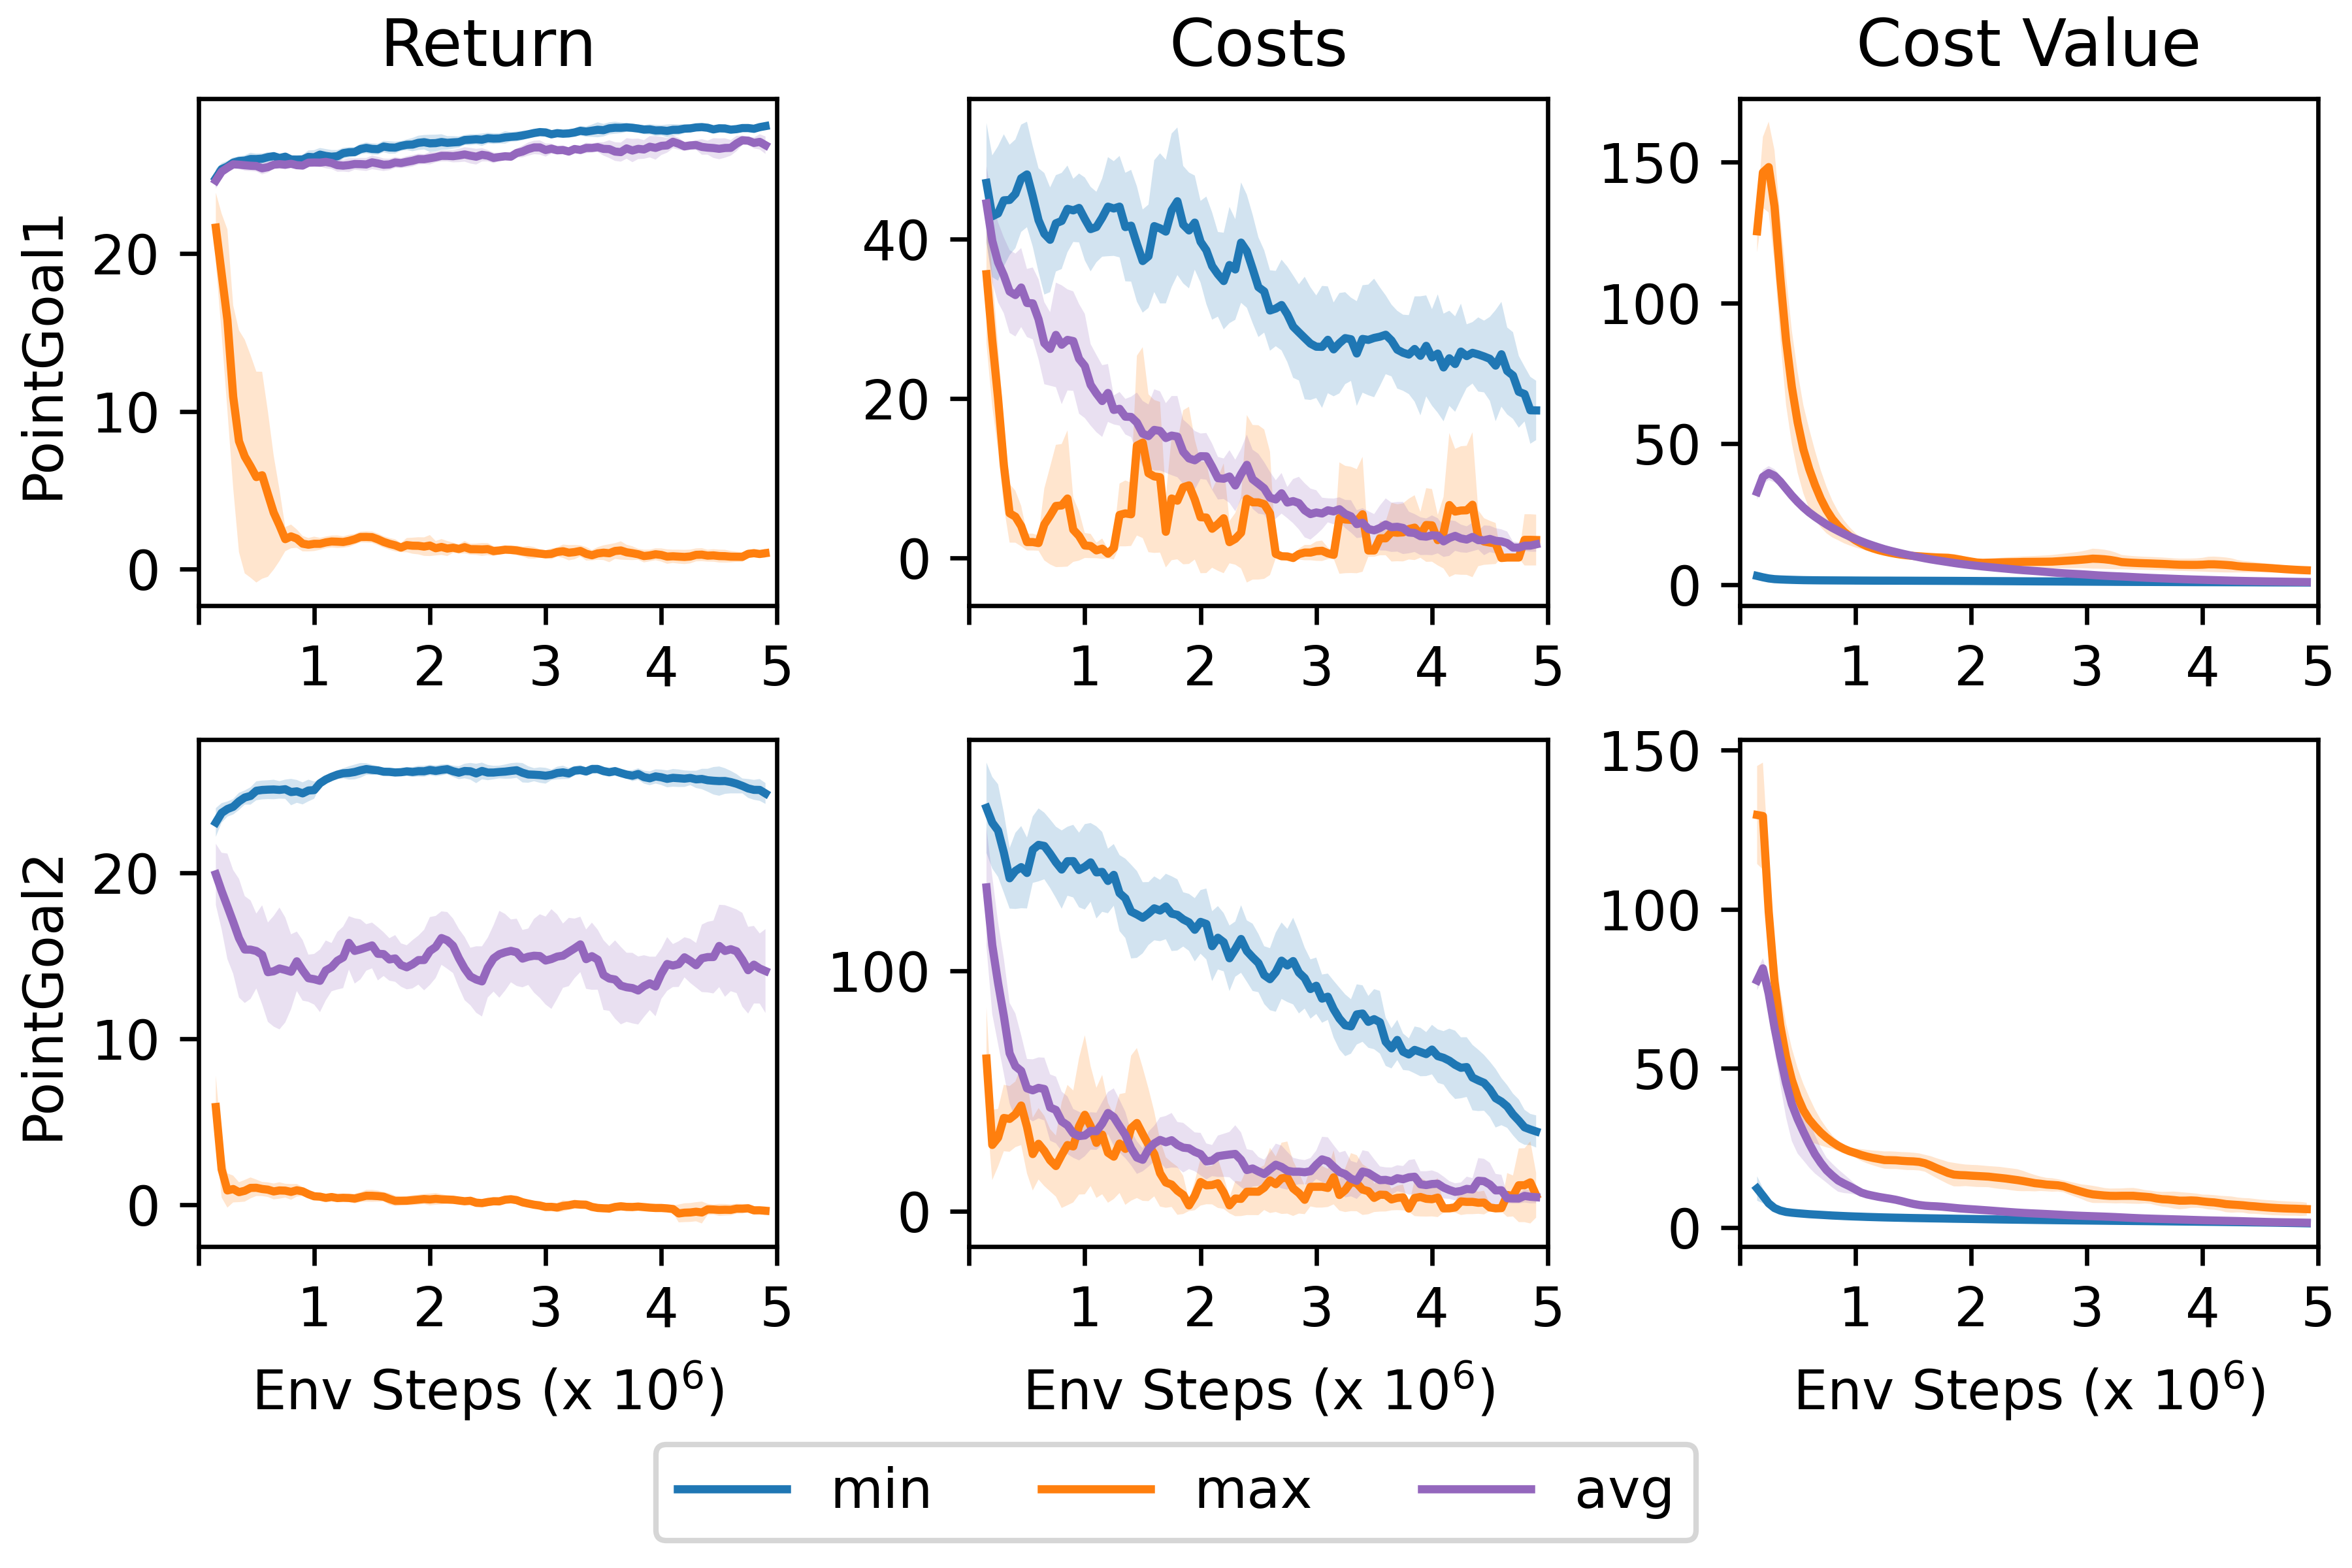
\includegraphics[width=0.95\linewidth]{cvaltarg.png}
    \caption{Сравнение способов агрегации ансамбля функций оценки долгосрочной стоимости.}
    \label{fig:synopsis_cvaltarg}
\end{figure}

Дополнительно проводится исследование размера ансамбля и схемы подвыборки функций оценки долгосрочной стоимости. Результаты показывают, что оценка одной функцией недостаточно устойчива, поскольку отдельная функция может давать смещённые оценки риска. Увеличение размера подвыборки снижает число нарушений безопасности, однако чрезмерное увеличение ансамбля не даёт существенного дополнительного выигрыша. На основе экспериментов выбрана схема $5 \times 5$ с усреднением, обеспечивающая достаточно точную оценку риска без заметного ухудшения целевой эффективности. Результаты абляционного исследования размера ансамбля и подвыборки функций оценки долгосрочной стоимости приведены на рис.~\ref{fig:synopsis_ensembles}.

\begin{figure}[ht]
    \centering
    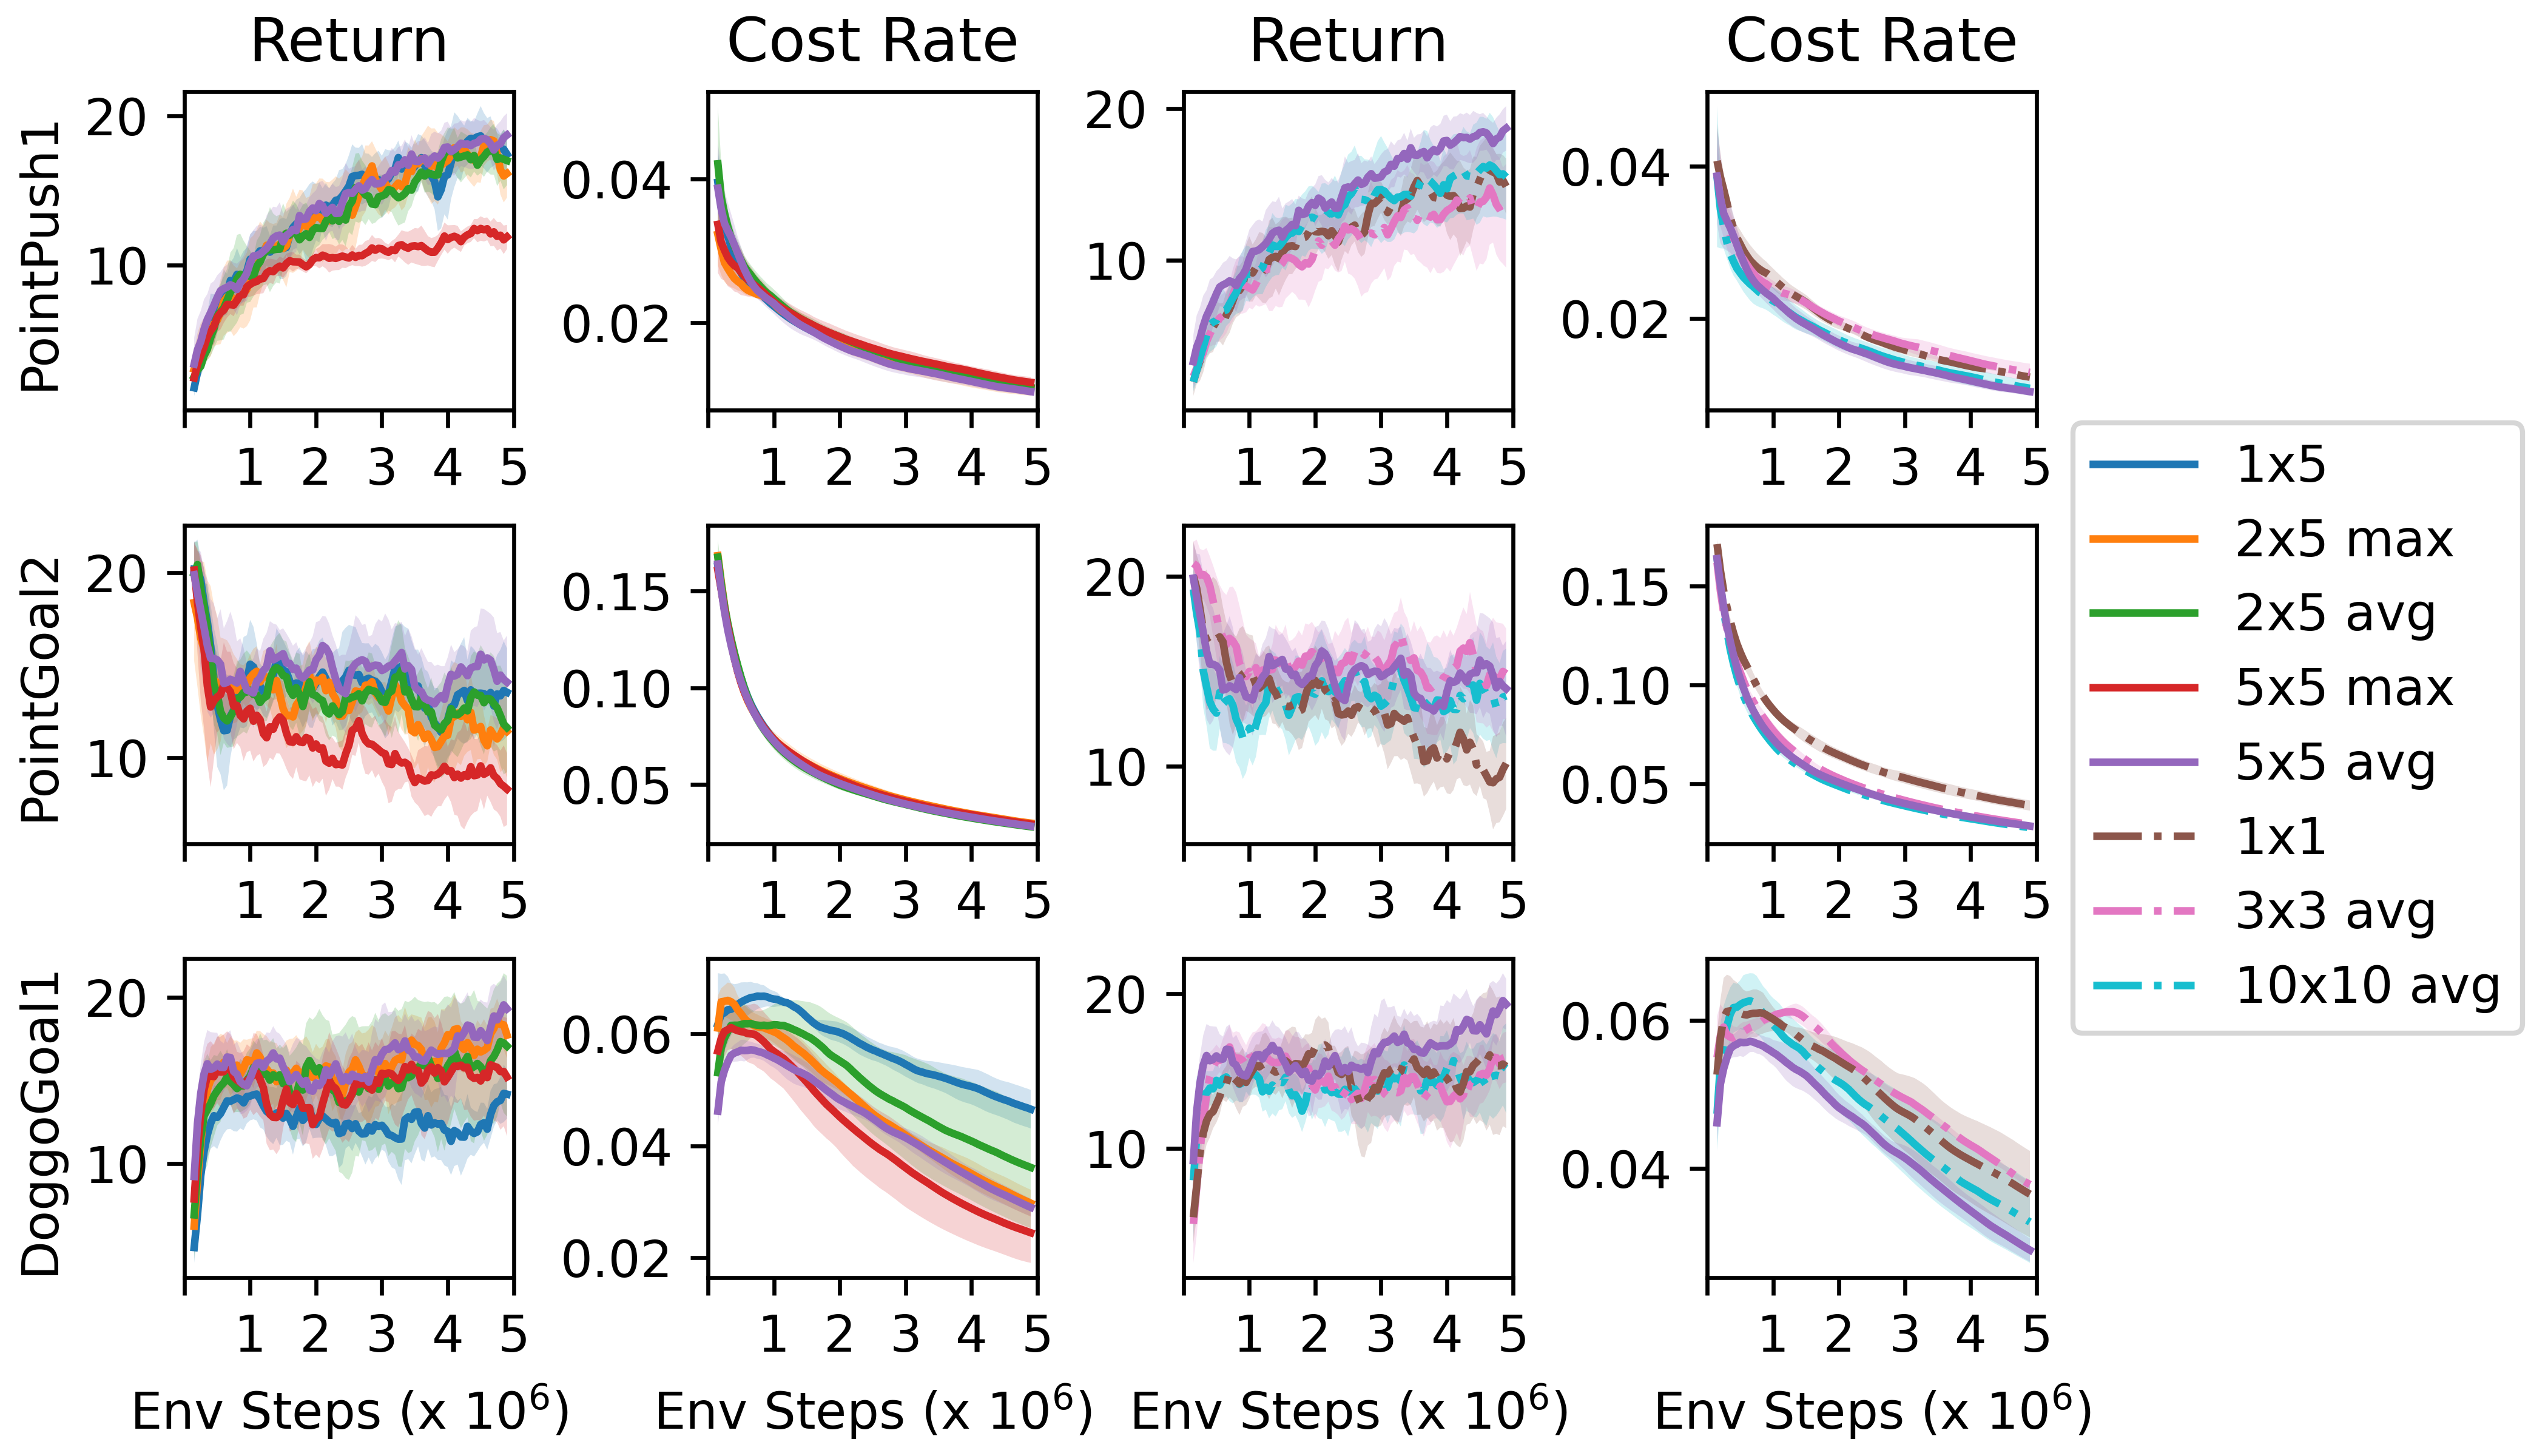
\includegraphics[width=0.95\linewidth]{ensembles.png}
    \caption{Абляционное исследование размера ансамбля и подвыборки функций оценки долгосрочной стоимости.}
    \label{fig:synopsis_ensembles}
\end{figure}

%Также в главе обсуждается различие между локальной и глобальной оценкой стоимости. Локальная оценка учитывает только ближайшие предсказанные штрафы и может обнаруживать риск слишком поздно, особенно при разреженных штрафных сигналах. Глобальная оценка дополняет сумму ближайших предсказанных штрафов оценкой долгосрочной стоимости, что позволяет учитывать риск за пределами короткого горизонта планирования. Однако такой подход требует устойчивого обучения функций оценки долгосрочной стоимости. Этот анализ показывает, что безопасное исследование в обучении с подкреплением на основе модели мира зависит от качества долгосрочной оценки риска внутри модели мира.

Полученные результаты показывают, что эффективность безопасного исследования в обучении с подкреплением на основе модели мира определяется не только наличием модели мира или планировщика, но и способом построения функций оценки долгосрочной стоимости. Устойчивая ансамблевая оценка долгосрочной стоимости позволяет агенту исследовать среду активнее, чем чрезмерно консервативные методы, и безопаснее, чем методы с оптимистичной недооценкой риска.

В \underline{\textbf{третьей главе}} рассматривается интеграция иерархического подхода в задачу безопасного исследования среды. Основная проблема, решаемая в главе, состоит в том, что неиерархические безопасные стратегии в задачах с большим горизонтом часто становятся чрезмерно консервативными: они уменьшают число нарушений безопасности, но хуже исследуют среду и не находят траектории к целевому состоянию. Для решения этой проблемы предложен метод SG-Safe, в котором генерация промежуточных подцелей используется для улучшения исследовательских способностей безопасной стратегии. Иерархическая структура применяется на этапе обучения, однако на этапе исполнения используется только итоговая безопасная стратегия, что позволяет избежать дополнительных вычислительных затрат и планирования во время исполнения.

\begin{figure}[ht]
    \centering
    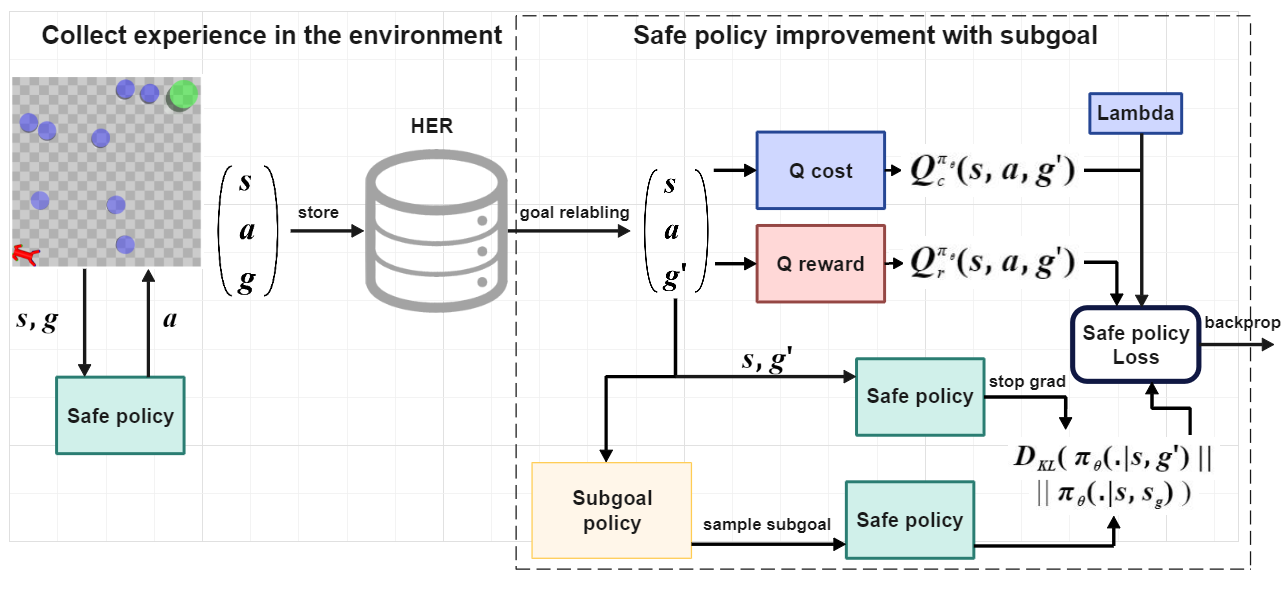
\includegraphics[width=0.95\linewidth]{method_scheme_3.png}
    \caption{Схема метода SG-Safe.}
    \label{fig:synopsis_sgsafe_scheme}
\end{figure}

Метод SG-Safe состоит из двух связанных компонент: безопасной стратегии и стратегии генерации подцелей. Безопасная стратегия реализуется на основе SAC-Lagrangian: для неё обучаются функции полезности по награде и стоимости, а множитель Лагранжа регулирует вклад штрафа за нарушение ограничений безопасности. Таким образом, стратегия обучается максимизировать достижение цели и одновременно ограничивать накопленную стоимость. Стратегия генерации подцелей используется для разбиения задачи с большим горизонтом на более короткие промежуточные переходы. Она генерирует подцели, которые направляют обучение безопасной стратегии к более информативным областям пространства состояний. При этом подцели не являются жёсткими командами: агент не обязан точно достигать каждую подцель, они используются как дополнительный обучающий сигнал, смещающий распределение действий в сторону более полезных траекторий.

Для повышения эффективности обучения в задачах с разреженной наградой в SG-Safe используется буфер с переиспользованием опыта и подстановкой достигнутых целей (Hindsight Experience Replay, HER). Опыт собирается безопасной стратегией и сохраняется в буфер HER, после чего цели в переходах переопределяются с использованием достигнутых состояний. Это позволяет получать дополнительные обучающие сигналы даже из неуспешных эпизодов. Далее из буфера HER выбираются переходы для обновления критика вознаграждения, критика стоимости, безопасной стратегии и стратегии генерации подцелей. Итоговая функция обновления безопасной стратегии включает три части: максимизацию ожидаемой награды, штраф за ожидаемую стоимость и регуляризатор, направляющий стратегию в сторону действий, согласованных с промежуточной подцелью. После завершения обучения стратегия подцелей не используется, а действие выбирается только безопасной стратегией. Общая схема метода приведена на рис.~\ref{fig:synopsis_sgsafe_scheme}.

Экспериментальная проверка SG-Safe проводилась на средах Safety Gym и POLAMP. В Safety Gym метод сравнивался с SAC, SAC-Lagrangian, CPO, L-RRT и вариантом SG-NoSafe, в котором подцели используются без безопасной оптимизации. Основной результат состоит в том, что SG-Safe повышает успешность выполнения задачи по сравнению с неиерархическими методами безопасного обучения с подкреплением при сохранении низкого уровня столкновений. В среднем по Safety Gym метод достигает доли успешных эпизодов $0.87$ при частоте столкновений $0.03$, тогда как SAC-Lagrangian достигает доли успешных эпизодов $0.40$ при частоте столкновений $0.05$. Это показывает, что подцели улучшают исследование безопасной стратегии, не разрушая баланс между достижением цели и безопасностью. Численные результаты приведены в табл.~\ref{tab:synopsis_sgsafe_sg}.

\begin{table}[ht]
\centering
\caption{Результаты на Safety Gym (SR~--- success rate, доля успешных эпизодов; CR~--- collision rate, частота столкновений; MTSC~--- episode cumulative safety cost, накопленная стоимость безопасности за эпизод). \textit{Среднее}~--- усреднение по средам Point, Car, Doggo и Sweeps.}
\label{tab:synopsis_sgsafe_sg}
\small
\setlength{\tabcolsep}{4pt}
\renewcommand{\arraystretch}{1.05}
\begin{tabularx}{\linewidth}{@{}>{\raggedright\arraybackslash}X >{\centering\arraybackslash}p{1.05cm} >{\centering\arraybackslash}p{1.05cm} >{\centering\arraybackslash}p{1.25cm}@{}}
\toprule
\multicolumn{4}{@{}l@{}}{\textit{Среднее} --- Point, Car, Doggo, Sweeps} \\
\midrule
Метод & SR$\uparrow$ & CR$\downarrow$ & MTSC$\downarrow$ \\
\midrule
SG-Safe & 0.87 & 0.03 & 13.7 \\
SG-NoSafe & 0.85 & 0.14 & 29.9 \\
L-RRT & 0.97 & 0.03 & 26.5 \\
SAC-LAG & 0.40 & 0.05 & 12.8 \\
SAC & 0.39 & 0.28 & 23.3 \\
CPO & 0.51 & 0.44 & 117.1 \\
\bottomrule
\end{tabularx}
\end{table}

На POLAMP эффект иерархического обучения выражен сильнее, поскольку среда содержит длинные маршруты и узкие коридоры. На втором уровне POLAMP метод SG-Safe достигает доли успешных эпизодов $0.88$ и частоты столкновений $0.03$, тогда как L-RRT получает долю успешных эпизодов $0.12$ и частоту столкновений $0.66$. При этом L-RRT требует планирования во время исполнения, а SG-Safe не использует планирование после обучения. В среднем по POLAMP метод достигает доли успешных эпизодов около $0.90$ при частоте столкновений около $0.03$, что подтверждает вклад генерации подцелей в безопасное исследование навигационных задач с большим горизонтом. Результаты сравнения приведены в табл.~\ref{tab:synopsis_sgsafe_polamp}.

\begin{table}[ht]
\centering
\caption{Сравнение SG-Safe с baseline-методами на POLAMP (SR~--- success rate, доля успешных эпизодов; CR~--- collision rate, частота столкновений; MTSC~--- episode cumulative safety cost, накопленная стоимость безопасности за эпизод). Показаны усреднённые по Level~1 и Level~2 результаты (Avg.). Лучшие значения выделены жирным. Результаты: среднее~$\pm$~СКО.}
\label{tab:synopsis_sgsafe_polamp}
\small
\setlength{\tabcolsep}{4pt}
\renewcommand{\arraystretch}{1.05}
\begin{tabularx}{\linewidth}{@{}>{\raggedright\arraybackslash}X >{\centering\arraybackslash}p{2.05cm} >{\centering\arraybackslash}p{2.05cm} >{\centering\arraybackslash}p{2.05cm}@{}}
\toprule
\multicolumn{4}{@{}l@{}}{\textit{Avg.} --- среднее по Level~1 и Level~2} \\
\midrule
Метод & SR$\uparrow$ & CR$\downarrow$ & MTSC$\downarrow$ \\
\midrule
SG-Safe & $\mathbf{0.897 \pm 0.026}$ & $0.028 \pm 0.010$ & $3.335 \pm 1.327$ \\
SAC-LAG & $0.364 \pm 0.006$ & $\mathbf{0.017 \pm 0.005}$ & $4.042 \pm 1.530$ \\
SAC & $0.305 \pm 0.020$ & $\mathbf{0.017 \pm 0.010}$ & $8.153 \pm 2.192$ \\
SAC-NCMP & $0.214 \pm 0.000$ & $0.787 \pm 0.000$ & $1.119 \pm 0.012$ \\
SAC-RCBF & $0.176 \pm 0.017$ & $0.145 \pm 0.017$ & $6.541 \pm 1.788$ \\
ADVICE & $0.000 \pm 0.000$ & $0.021 \pm 0.000$ & $\mathbf{0.021 \pm 0.000}$ \\
L-RRT & $0.338 \pm 0.080$ & $0.507 \pm 0.084$ & $10.245 \pm 2.289$ \\
\bottomrule
\end{tabularx}
\end{table}

Полученные результаты показывают, что SG-Safe позволяет перенести иерархическую структуру в фазу обучения безопасной стратегии, не сохраняя её как обязательный планировщик на этапе применения. Это делает метод применимым в задачах, где агент должен исследовать среду при ограничении числа небезопасных действий, но при этом не может полагаться на полную карту среды, точную модель динамики или вычислительно затратное планирование во время исполнения.

В \underline{\textbf{четвёртой главе}} рассматривается развитие иерархического безопасного обучения с подкреплением за счёт использования модели мира. Если метод SG-Safe применяет подцели как способ улучшить исследование безопасной стратегии, то метод ITES решает более сильную задачу: обеспечить безопасность как при выборе промежуточных подцелей, так и при их достижении низкоуровневой стратегией. Основная проблема, рассматриваемая в главе, состоит в том, что существующие методы безопасного обучения с подкреплением плохо работают в задачах с большим горизонтом: они либо нарушают ограничения безопасности, либо становятся чрезмерно консервативными и не достигают цели. Эта проблема особенно выражена в задачах, где агенту требуется выполнить длинную последовательность действий, управлять системой с высокой размерностью или обучаться при разреженной награде. Для решения этой проблемы предложен метод ITES (Imagine To Ensure Safety in Hierarchical Reinforcement Learning), объединяющий иерархическую структуру, модель стоимости и модель мира. Общая схема метода приведена на рис.~\ref{fig:synopsis_ites_scheme}.

\begin{figure}[ht]
    \centering
    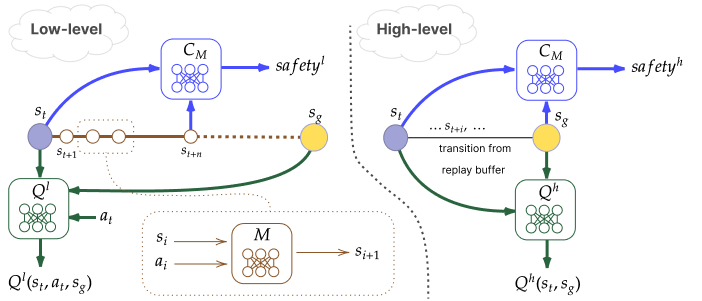
\includegraphics[width=0.95\linewidth]{learning_scheme_1.png}
    \caption{Схема обучения ITES. Слева: модель стоимости $C_M$ и модель мира $M$ обеспечивают безопасность низкоуровневой стратегии. Справа: модель стоимости $C_M$ и высокоуровневый критик стоимости используются для генерации безопасных подцелей.}
    \label{fig:synopsis_ites_scheme}
\end{figure}

Метод ITES строится на иерархической архитектуре с двумя стратегиями: высокоуровневой стратегией $\pi^h$, генерирующей промежуточные подцели, и низкоуровневой стратегией $\pi^l$, выбирающей действия для достижения текущей подцели. В качестве базовой иерархической структуры используется HRAC, где сеть смежности ограничивает пространство подцелей состояниями, достижимыми за ограниченное число шагов. Для обеспечения безопасности на верхнем уровне в ITES вводятся два дополнительных компонента: модель стоимости и высокоуровневый критик стоимости. Модель стоимости оценивает, является ли выбранная подцель безопасной, а высокоуровневый критик стоимости оценивает ожидаемую долгосрочную стоимость выбора этой подцели. Это необходимо, поскольку локально безопасная подцель может быть труднодостижимой и приводить к небезопасной траектории при её достижении. Поэтому высокоуровневая стратегия обучается выбирать подцели, которые одновременно полезны для достижения конечной цели, достижимы и не приводят к превышению допустимого уровня стоимости.

Для обеспечения безопасности на нижнем уровне ITES использует модель мира. Низкоуровневая стратегия генерирует действие для достижения текущей подцели, после чего модель мира предсказывает короткую воображаемую траекторию. Затем модель стоимости оценивает безопасность этой траектории. Такой подход позволяет уменьшить вероятность небезопасных действий ещё до их выполнения в среде. При этом в методе используется не полный суммарный штраф по длинной воображаемой траектории, а случайно выбранный шаг такой траектории. Это снижает накопление ошибки модели мира и уменьшает риск нестабильного обучения. Для обучения модели стоимости используется сбалансированный буфер воспроизведения опыта, содержащий безопасные и небезопасные состояния, а для модели мира~--- лёгкий ансамбль предиктивных моделей, предсказывающих следующее состояние.

Экспериментальная проверка ITES проводилась на робототехнических задачах с большим горизонтом SafeAntMaze и SafePusher, а также на задачах с маленьким горизонтом SafetyGym. В SafeAntMaze и SafePusher метод сравнивался с алгоритмами CUP, FOCOPS, TD3LAG, PPOLAG, SafeDreamer, а также с иерархическими методами сравнения HRAC и HRAC-LAG. Результаты показывают, что существующие методы безопасного обучения с подкреплением часто имеют мало нарушений ограничений не потому, что успешно решают задачу безопасно, а потому что не достигают цели и остаются в консервативном поведении. Например, в SafeAntMaze C-shape методы SafeDreamer, CUP и FOCOPS имеют нулевую долю успешных эпизодов, тогда как ITES достигает доли успешных эпизодов $0.88$ при стоимости $15.2$. В SafeAntMaze W-shape ITES достигает доли успешных эпизодов $0.35$, тогда как большинство неиерархических методов имеет нулевую успешность. В SafePusher ITES достигает доли успешных эпизодов $0.42$ при стоимости $12.8$, в то время как SafeDreamer и другие неиерархические методы практически не решают задачу. Итоговые значения на задачах с большим горизонтом приведены в табл.~\ref{tab:synopsis_ites_long}.

\begin{table}[ht]
\centering
\caption{Итоговые результаты на SafeAntMaze и SafePusher (SAM-C~--- SafeAntMaze C-shape; SAM-W~--- SafeAntMaze W-shape; SR~--- success rate, доля успешных эпизодов; Cost~--- cumulative cost, накопленная стоимость за эпизод; $d$~--- cost limit, допустимый бюджет стоимости). Зелёным выделены методы с Cost~$\leq d$, красным~--- с Cost~$> d$. Лучшие значения в группе выделены жирным. Результаты: среднее~$\pm$~СКО по 5 seed.}
\label{tab:synopsis_ites_long}
\footnotesize
\setlength{\tabcolsep}{4pt}
\renewcommand{\arraystretch}{1.12}
\begin{tabularx}{\linewidth}{@{}>{\raggedright\arraybackslash}X >{\centering\arraybackslash}p{2.15cm} >{\centering\arraybackslash}p{2.55cm}@{}}
\toprule
Метод & SR$\uparrow$ & Cost$\downarrow$ \\
\midrule
\multicolumn{3}{@{}l@{}}{\textbf{SAM-C} (SafeAntMaze C-shape)} \\
\rowcolor{green!15} ITES & $\mathbf{0.88 \pm 0.01}$ & $15.2 \pm 17.3$ \\
\rowcolor{green!15} SafeDreamer & $0$ & $13.0 \pm 18.11$ \\
\rowcolor{green!15} CUP & $0$ & $\mathbf{6.8 \pm 22.4}$ \\
\rowcolor{green!15} FOCOPS & $0$ & $19.4 \pm 50.9$ \\
\rowcolor{red!12} TD3L/R & $0.38 \pm 0.04$ & $83.6 \pm 37.2$ \\
\rowcolor{red!12} PPOLAG & $0.20 \pm 0.20$ & $41.2 \pm 1.1$ \\
\rowcolor{red!12} TD3LAG & $0.13 \pm 0.33$ & $133.45 \pm 184.4$ \\
\addlinespace[0.3em]
\multicolumn{3}{@{}l@{}}{\textbf{SAM-W} (SafeAntMaze W-shape)} \\
\rowcolor{green!15} ITES & $\mathbf{0.35 \pm 0.05}$ & $183.0 \pm 16.5$ \\
\rowcolor{green!15} TD3L/R & $0.05 \pm 0.02$ & $154.0 \pm 13.5$ \\
\rowcolor{green!15} CUP & $0$ & $\mathbf{103.5 \pm 21.5}$ \\
\rowcolor{green!15} FOCOPS & $0$ & $141.0 \pm 26.0$ \\
\rowcolor{green!15} TD3LAG & $0$ & $128.68 \pm 210.0$ \\
\rowcolor{green!15} PPOLAG & $0$ & $105.0 \pm 20.1$ \\
\rowcolor{red!12} SafeDreamer & $0$ & $216.3 \pm 199.0$ \\
\addlinespace[0.3em]
\multicolumn{3}{@{}l@{}}{\textbf{Pusher} (SafePusher)} \\
\rowcolor{green!15} ITES & $\mathbf{0.42 \pm 0.02}$ & $\mathbf{12.8 \pm 0.87}$ \\
\rowcolor{green!15} SafeDreamer & $0$ & $6.7 \pm 2.7$ \\
\rowcolor{red!12} TD3LAG & $0.05 \pm 0.03$ & $54.72 \pm 3.16$ \\
\rowcolor{red!12} CUP & $0.01$ & $46.14 \pm 0.42$ \\
\rowcolor{red!12} FOCOPS & $0$ & $55.83 \pm 1.67$ \\
\rowcolor{red!12} PPOLAG & $0$ & $51.25 \pm 1.25$ \\
\bottomrule
\end{tabularx}
\end{table}

Дополнительно ITES сравнивался с HRAC и HRAC-LAG, что позволяет оценить вклад компонентов безопасности, а не только самой иерархической структуры. В SafeAntMaze C-shape иерархические методы могут достигать сопоставимой успешности, однако ITES снижает стоимость нарушений за счёт совместного использования модели стоимости и модели мира. В SafePusher метод показывает более высокую успешность, что подтверждает пользу проверки безопасности через модель мира в задачах с более сложной динамикой и высокоразмерным управлением. На задачах с малым горизонтом SafetyGym метод также сохраняет конкурентоспособность: в PointGoal1 ITES достигает награды $19.6$ при стоимости $32.83$, в CarGoal1~--- награды $18.3$ при стоимости $21.72$, а в sparse PointGoal~--- награды $8.64$ при стоимости $33.46$. Во всех этих случаях стоимость остаётся ниже заданного бюджета $d = 40$, что показывает способность метода сохранять баланс между безопасностью и эффективностью не только в задачах с большим горизонтом, но и в более стандартных задачах безопасного обучения с подкреплением. Итоговые значения на задачах SafetyGym приведены в табл.~\ref{tab:synopsis_ites_sg}.

\begin{table}[ht]
\centering
\caption{Итоговые результаты на SafetyGym (PG1~--- PointGoal1; CG1~--- CarGoal1; PGs~--- PointGoal1 sparse; Reward~--- reward, награда; Cost~--- cumulative cost, накопленная стоимость за эпизод; $d = 40$~--- cost limit, допустимый бюджет стоимости). Лучшие значения Reward в группе выделены жирным. Результаты: среднее~$\pm$~СКО по 5 seed.}
\label{tab:synopsis_ites_sg}
\setlength{\tabcolsep}{5pt}
\renewcommand{\arraystretch}{1.08}
\begin{tabularx}{\linewidth}{@{}>{\raggedright\arraybackslash}X >{\centering\arraybackslash}p{2.35cm} >{\centering\arraybackslash}p{2.75cm}@{}}
\toprule
Метод & Reward$\uparrow$ & Cost$\downarrow$ \\
\midrule
\multicolumn{3}{@{}l@{}}{\textbf{PG1} (PointGoal1)} \\
ITES & $\mathbf{19.6 \pm 0.46}$ & $32.83 \pm 1.97$ \\
TD3LAG & $15.75 \pm 0.39$ & $56.22 \pm 0.85$ \\
FOCOPS & $14.97 \pm 9.01$ & $33.72 \pm 42.24$ \\
CUP & $14.42 \pm 6.74$ & $19.02 \pm 20.08$ \\
PPOLAG & $12.96 \pm 6.95$ & $25.80 \pm 34.99$ \\
SafeDreamer & $12.0 \pm 4.0$ & $10.3 \pm 9.5$ \\
\addlinespace[0.3em]
\multicolumn{3}{@{}l@{}}{\textbf{CG1} (CarGoal1)} \\
ITES & $\mathbf{18.3 \pm 0.03}$ & $21.72 \pm 0.59$ \\
FOCOPS & $15.23 \pm 10.76$ & $31.66 \pm 93.51$ \\
PPOLAG & $13.27 \pm 9.26$ & $21.72 \pm 32.06$ \\
TD3LAG & $8.21 \pm 6.88$ & $53.7 \pm 9.45$ \\
SafeDreamer & $6.6 \pm 1.2$ & $0$ \\
CUP & $6.14 \pm 6.97$ & $36.12 \pm 89.56$ \\
\addlinespace[0.3em]
\multicolumn{3}{@{}l@{}}{\textbf{PGs} (PointGoal1 sparse)} \\
ITES & $\mathbf{8.64 \pm 0.38}$ & $33.46 \pm 1.47$ \\
FOCOPS & $7.635 \pm 0.2$ & $22.9 \pm 1.5$ \\
PPOLAG & $6.85 \pm 0.76$ & $32.645 \pm 5.9$ \\
CUP & $1.755 \pm 0.95$ & $12.925 \pm 5.3$ \\
SafeDreamer & $0.5 \pm 0.5$ & $3.22 \pm 2.34$ \\
TD3LAG & $0.07 \pm 0.01$ & $64.7 \pm 1.91$ \\
\bottomrule
\end{tabularx}
\end{table}

Полученные результаты показывают, что ITES решает основное ограничение неиерархических безопасных стратегий: неспособность эффективно исследовать и решать задачи с большим горизонтом при сохранении ограничений безопасности. Иерархическая структура позволяет разбивать исходную задачу на более короткие подзадачи, модель стоимости и высокоуровневый критик стоимости направляют генерацию подцелей в безопасные области, а модель мира снижает риск небезопасных действий низкоуровневой стратегии при достижении подцелей. Поэтому ITES можно рассматривать как развитие SG-Safe: если SG-Safe улучшает исследование безопасной стратегии через подцели, то ITES дополнительно вводит явный контроль безопасности подцелей и действий с использованием модели мира.

\underline{\textbf{Пятая глава}} посвящена бенчмарку Caged CrafText, предназначенному для оценки агентов в задачах безопасного обучения с подкреплением, где и цель, и ограничения задаются естественным языком. Глава продолжает линию диссертации от классического безопасного обучения с подкреплением с численной функцией стоимости к более общей мультимодальной постановке. Основная проблема состоит в том, что агент может корректно выполнить языковую инструкцию, но при этом нарушить ограничение поведения: израсходовать ресурс, атаковать запрещённый объект, приблизиться к опасной зоне или выполнить действия в неправильном порядке. Поэтому для оценки безопасных агентов недостаточно проверять только достижение цели; необходимо также проверять понимание и соблюдение текстового ограничения. В главе описывается бенчмарк Caged CrafText, расширяющий CrafText до постановки с естественно-языковыми ограничениями. В каждой задаче агент получает две текстовые инструкции: инструкцию цели и инструкцию ограничения безопасности.

Бенчмарк включает четыре типа ограничений: бюджетные, последовательные, математические и отношенческие. Эти ограничения проверяют разные способности агента: память, глубокое исследование среды, безопасное исследование, рассуждение и понимание естественного языка. Таксономия задач Caged CrafText приведена в табл.~\ref{tab:synopsis_caged_taxonomy}. Для оценки предложены два набора задач: отладочный набор задач, предназначенный для диагностики отдельных типов ошибок, и основной набор задач, предназначенный для общей оценки способности агента соблюдать языковые ограничения в разных задачах и при различных формулировках инструкций.

\begin{table}[ht]
\centering
\caption{Таксономия задач Caged CrafText и проверяемых способностей агента. В ограничениях используются пиктограммы: \synemj{food.png} (еда), \synemj{drink.png} (вода), \synemj{energy.png} (энергия), \synemj{health.png} (здоровье), \synemj{wood_sword.png} (деревянный меч), \synemj{tree.png} (дерево), \synemj{cow.png} (корова), \synemj{zombie.png} (зомби), \synemj{skeleton.png} (скелет). M~--- memory, память; DE~--- deep exploration, глубокое исследование; SE~--- safe exploration, безопасное исследование; R~--- reasoning, рассуждение; LU~--- language understanding, понимание языка.}
\label{tab:synopsis_caged_taxonomy}
\small
\setlength{\tabcolsep}{3pt}
\renewcommand{\arraystretch}{1.2}
\newlength{\synTaxScenarioW}
\newlength{\synTaxAbilityW}
\setlength{\synTaxScenarioW}{0.21\linewidth}
\setlength{\synTaxAbilityW}{0.075\linewidth}
\begin{tabularx}{\linewidth}{@{}>{\raggedright\arraybackslash}p{\synTaxScenarioW}>{\raggedright\arraybackslash}X *{5}{>{\centering\arraybackslash}p{\synTaxAbilityW}}@{}}
\toprule
\textbf{Сценарий} & \textbf{Ограничение} & \textbf{M} & \textbf{DE} & \textbf{SE} & \textbf{R} & \textbf{LU} \\
\midrule
\multirow{4}{=}{\parbox[t]{\synTaxScenarioW}{\raggedright Бюджетные}} &
Поддерживать \synemj{food.png} $\geq 5$ & $\checkmark$ & $\checkmark$ & $\checkmark$ & & \\
& Поддерживать \synemj{drink.png} $\geq 5$ & $\checkmark$ & $\checkmark$ & $\checkmark$ & & \\
& Поддерживать \synemj{energy.png} $\geq 5$ & & & $\checkmark$ & & \\
& Поддерживать \synemj{health.png} $\geq 5$ & $\checkmark$ & $\checkmark$ & $\checkmark$ & $\checkmark$ & \\
\midrule
\multirow{3}{=}{\parbox[t]{\synTaxScenarioW}{\raggedright Последовательные}} &
Не атаковать \synemj{zombie.png}\synemj{skeleton.png} без \synemj{wood_sword.png} & & $\checkmark$ & $\checkmark$ & $\checkmark$ & \\
& Не спать рядом с \synemj{zombie.png}\synemj{skeleton.png} & & & $\checkmark$ & $\checkmark$ & \\
& При \synemj{health.png} $\leq 4$ избегать \synemj{zombie.png}\synemj{skeleton.png} & & & $\checkmark$ & $\checkmark$ & \\
\midrule
\multirow{2}{=}{\parbox[t]{\synTaxScenarioW}{\raggedright Математические}} &
бюджет 20, $-10$ за убийство \synemj{cow.png} & $\checkmark$ & & $\checkmark$ & $\checkmark$ & \\
& бюджет 50, $-10$ за рубку \synemj{tree.png} & $\checkmark$ & & $\checkmark$ & $\checkmark$ & \\
\midrule
\multirow{3}{=}{\parbox[t]{\synTaxScenarioW}{\raggedright Отношенческие}} &
Избегать \synemj{zombie.png}\synemj{skeleton.png} в пределах 3 клеток & $\checkmark$ & & $\checkmark$ & $\checkmark$ & \\
& Найти источник \synemj{drink.png} & $\checkmark$ & $\checkmark$ & $\checkmark$ & & \\
& Найти источник \synemj{food.png} & $\checkmark$ & $\checkmark$ & $\checkmark$ & & \\
\midrule
\multicolumn{2}{>{\raggedright\arraybackslash}X}{\textbf{Бюджетные (все):} все бюджетные ограничения} & $\checkmark$ & $\checkmark$ & $\checkmark$ & $\checkmark$ & \\
\multicolumn{2}{>{\raggedright\arraybackslash}X}{\textbf{Последовательные (все):} все последовательные ограничения} & & $\checkmark$ & $\checkmark$ & $\checkmark$ & \\
\multicolumn{2}{>{\raggedright\arraybackslash}X}{\textbf{Математические (все):} все математические ограничения} & $\checkmark$ & & $\checkmark$ & $\checkmark$ & \\
\multicolumn{2}{>{\raggedright\arraybackslash}X}{\textbf{Отношенческие (все):} все отношенческие ограничения} & $\checkmark$ & $\checkmark$ & $\checkmark$ & $\checkmark$ & \\
\midrule
\multicolumn{2}{>{\raggedright\arraybackslash}X}{\textbf{Caged:} все ограничения и перефразировки} & $\checkmark$ & $\checkmark$ & $\checkmark$ & $\checkmark$ & $\checkmark$ \\
\bottomrule
\end{tabularx}
\end{table}

Экспериментальная часть главы включает сравнение нескольких базовых подходов: PPO, PPO-LAG, PPO-Cost и LLM-агента. PPO используется как агент, оптимизирующий только награду и игнорирующий стоимость. PPO-LAG использует лагранжеву оптимизацию ограничения, а PPO-Cost добавляет стоимость непосредственно в функцию награды. Для всех обучаемых подходов текст цели и текст ограничения кодируются при помощи BERT, после чего используются стратегией агента. Сравнение базовых методов приведено в табл.~\ref{tab:synopsis_caged_results}.

\begin{table}[ht]
\centering
\caption{Сравнение базовых алгоритмов и LLM-агента на бенчмарке Caged CrafText (R~--- reward, награда; C~--- cost, штраф за нарушение ограничений). Лучшие результаты в каждом столбце выделены жирным. Результаты усреднены по 5 случайным seed.}
\label{tab:synopsis_caged_results}
\scriptsize
\setlength{\tabcolsep}{2pt}
\renewcommand{\arraystretch}{1.05}
\resizebox{\linewidth}{!}{%
\begin{tabular}{@{}>{\raggedright\arraybackslash}p{4.6cm} c c @{\hspace{0.8em}} c c @{\hspace{0.8em}} c c @{\hspace{0.8em}} c c@{}}
\hline
 & \multicolumn{2}{c}{\textbf{PPO}} & \multicolumn{2}{c}{\textbf{PPO-LAG}} & \multicolumn{2}{c}{\textbf{PPO-Cost}} & \multicolumn{2}{c}{\textbf{LLM}} \\
\cline{2-3} \cline{4-5} \cline{6-7} \cline{8-9}
 & R$\uparrow$ & C$\downarrow$ & R$\uparrow$ & C$\downarrow$ & R$\uparrow$ & C$\downarrow$ & R$\uparrow$ & C$\downarrow$ \\
\hline
\multicolumn{9}{@{}l@{}}{\textbf{Budgetary} ($d = 0.1$)} \\
\hspace{0.4cm} Maintain \synemj{food.png} $\geq 5$ & \textbf{0.22} & 17.16 & 0.04 & 0.75 & 0.11 & 0.12 & 0.19 & 28.7 \\
\hspace{0.4cm} Maintain \synemj{drink.png} $\geq 5$ & \textbf{0.22} & 57.94 & 0.04 & 1.12 & 0.05 & 0.73 & 0.19 & 31.2 \\
\hspace{0.4cm} Maintain \synemj{energy.png} $\geq 5$ & 0.20 & 20.57 & \textbf{0.22} & 0.10 & 0.20 & \textbf{0.01} & 0.19 & 26.4 \\
\hspace{0.4cm} Maintain \synemj{health.png} $\geq 5$ & \textbf{0.23} & 22.12 & 0.02 & \textbf{0.06} & 0.08 & 1.32 & 0.19 & 29.8 \\
\hline
\multicolumn{9}{@{}l@{}}{\textbf{Sequential} ($d = 0.1$)} \\
\hspace{0.4cm} Don't attack \synemj{zombie.png}\synemj{skeleton.png} w/o \synemj{wood_sword.png} & \textbf{0.23} & 1.76 & 0.20 & 0.10 & 0.20 & \textbf{0.00} & 0.19 & 18.3 \\
\hspace{0.4cm} Don't sleep nearby \synemj{zombie.png}\synemj{skeleton.png} & 0.20 & 8.12 & \textbf{0.23} & 1.06 & 0.20 & \textbf{0.00} & 0.19 & 22.6 \\
\hspace{0.4cm} When \synemj{health.png} $\leq 4$, avoid \synemj{zombie.png}\synemj{skeleton.png} & \textbf{0.23} & 9.54 & 0.03 & 1.21 & 0.09 & 0.93 & 0.19 & 24.1 \\
\hline
\multicolumn{9}{@{}l@{}}{\textbf{Mathematical} ($d = 0.1$)} \\
\hspace{0.4cm} 20 budget, $-10$ for killing \synemj{cow.png} & 0.22 & 111.88 & \textbf{0.24} & 0.10 & 0.18 & 0.04 & 0.19 & 18.3 \\
\hspace{0.4cm} 50 budget, $-10$ for chopping \synemj{tree.png} & 0.21 & 114.81 & 0.21 & 0.11 & 0.20 & 0.08 & 0.19 & 8.3 \\
\hline
\multicolumn{9}{@{}l@{}}{\textbf{Relational} ($d = 10$)} \\
\hspace{0.4cm} Avoid \synemj{zombie.png}\synemj{skeleton.png} within 3 cells & \textbf{0.21} & 51.96 & \textbf{0.11} & 9.55 & 0.04 & 7.72 & 0.18 & 47.3 \\
\hspace{0.4cm} Find source of \synemj{drink.png} & \textbf{0.21} & 95.96 & 0.03 & 11.80 & 0.04 & 12.09 & 0.18 & 52.6 \\
\hspace{0.4cm} Find source of \synemj{food.png} & \textbf{0.22} & 20.67 & 0.03 & 13.40 & 0.04 & 12.24 & 0.19 & 49.8 \\
\hline
\textbf{Budgetary All} ($d = 0.1$) & \textbf{0.23} & 11.38 & 0.05 & 0.36 & 0.11 & 0.12 & 0.19 & 40.1 \\
\textbf{Sequential All} ($d = 0.1$) & \textbf{0.24} & 7.65 & 0.05 & 1.02 & 0.08 & 0.82 & 0.19 & 22.7 \\
\textbf{Mathematical All} ($d = 0.1$) & \textbf{0.23} & 110.42 & \textbf{0.24} & \textbf{0.10} & 0.18 & 0.05 & 0.19 & 16.9 \\
\textbf{Relational All} ($d = 10$) & \textbf{0.22} & 31.36 & 0.11 & 11.69 & 0.04 & 8.18 & 0.18 & 15.2 \\
\hline
\textbf{Caged} ($d = 0.1$) & \textbf{0.22} & 103.66 & 0.03 & 0.17 & 0.14 & 0.13 & \textbf{0.20} & 43.4 \\
\hline
\end{tabular}%
}
\end{table}

Результаты показывают несколько характерных ошибок. PPO достигает высокой награды почти во всех задачах, но систематически нарушает ограничения: например, на наборе Caged он получает награду $0.22$ при штрафе $103.66$. PPO-LAG существенно снижает стоимость, но часто становится чрезмерно консервативным и теряет способность решать задачу: на Caged он получает награду $0.03$ при штрафе $0.17$. PPO-Cost даёт более сбалансированное поведение в части задач, например на Caged достигает награду $0.14$ при штрафе $0.13$, но всё ещё не решает задачу устойчивого совмещения цели и языкового ограничения. На математических ограничениях PPO-LAG и PPO-Cost показывают лучшие результаты, что указывает на относительную простоту ограничений, связанных с явным численным бюджетом. Однако на бюджетных, последовательных и отношенческих ограничениях обучаемые методы часто либо нарушают ограничения, либо перестают эффективно исследовать среду.

Отдельно показано, что LLM-агент демонстрирует более стабильную способность к выполнению целевых инструкций: на разных категориях задач его награда остаётся около $0.18$--$0.20$. Однако стоимость остаётся высокой: на Caged LLM получает штраф $43.4$, на Budgetary All~--- $40.1$, на Sequential All~--- $22.7$. Это показывает, что LLM обладает полезными способностями к рассуждению и планированию, но страдает от проблем понимания среды: модель не всегда может связать текстовое ограничение с конкретными объектами, состояниями и безопасными действиями в среде.

Таким образом, эксперименты подтверждают, что Caged CrafText выявляет ограничения как классических методов безопасного обучения с подкреплением, так и LLM-агентов. Первые часто не обладают достаточными способностями к рассуждению, памяти и долгосрочному планированию, вторые лучше интерпретируют инструкцию, но недостаточно надёжно связывают её с динамикой среды. Это показывает необходимость разработки агентов, объединяющих безопасное исследование, мультимодальное восприятие, память, понимание среды и долгосрочное планирование.

\FloatBarrier
\pdfbookmark{Заключение}{conclusion}
\section*{Заключение}

Диссертационная работа посвящена разработке и исследованию методов безопасного обучения с подкреплением для задач, в которых агент должен одновременно исследовать среду, достигать целевой награды и соблюдать ограничения безопасности. Основное внимание уделено трём направлениям: использованию моделей мира для предварительной оценки последствий действий, иерархической декомпозиции поведения для задач с большим горизонтом и переходу к мультимодальной постановке, где цели и ограничения задаются естественным языком.

В работе проведён обзор современных методов безопасного обучения с подкреплением и показано, что существующие подходы сталкиваются с рядом ограничений. Неиерархические безопасные стратегии часто становятся чрезмерно консервативными и плохо решают задачи с большим горизонтом. Методы на основе моделей мира позволяют заранее оценивать последствия действий, но чувствительны к ошибкам модели и выбору порогов безопасности. Методы, использующие априорные знания о среде, могут обеспечивать более строгий контроль безопасности, однако требуют известных динамических моделей, явных функций ограничений или дополнительной информации о среде, что ограничивает их применимость в реальных робототехнических задачах.

В рамках направления безопасного обучения с подкреплением на основе модели мира исследован подход SPOWL, в котором модель мира используется для оценки награды, стоимости и долгосрочного риска кандидатных действий. Показано, что безопасное исследование должно учитывать не только мгновенную стоимость, но и оценки долгосрочной стоимости, позволяющие оценивать риск за пределами короткого горизонта планирования. Экспериментальный анализ показал, что способ агрегации ансамбля функций оценки долгосрочной стоимости существенно влияет на баланс между безопасностью и эффективностью: минимальная агрегация недооценивает риск, максимальная приводит к избыточной консервативности, а усреднение обеспечивает наиболее устойчивое поведение агента.

Для решения проблемы безопасного исследования в задачах с большим горизонтом разработан метод SG-Safe. Метод использует стратегию генерации промежуточных подцелей, которая применяется на этапе обучения и направляет безопасную стратегию к более информативным областям пространства состояний. При этом на этапе исполнения используется только итоговая безопасная стратегия, поэтому метод не требует онлайн-планирования и дополнительных вычислительных затрат. Эксперименты на Safety Gym и POLAMP показали, что SG-Safe повышает успешность решения навигационных задач при сохранении низкого уровня нарушений безопасности. В среднем на Safety Gym метод достигает доли успешных эпизодов $0.87$ при частоте столкновений $0.03$, а на POLAMP демонстрирует преимущество в задачах с длинными маршрутами и узкими коридорами.

Дальнейшее развитие иерархического подхода реализовано в методе ITES. В отличие от SG-Safe, метод ITES вводит явный контроль безопасности как на уровне генерации подцелей, так и на уровне их достижения. Верхнеуровневая стратегия генерирует промежуточные подцели с учётом модели стоимости и высокоуровневого критика стоимости, а низкоуровневая стратегия использует модель мира для проверки безопасности коротких воображаемых траекторий. Эксперименты на SafeAntMaze и SafePusher показали, что ITES превосходит неиерархические методы безопасного обучения с подкреплением в задачах с большим горизонтом, где многие методы сравнения либо нарушают ограничения, либо не достигают цели. В SafeAntMaze C-shape метод достигает доли успешных эпизодов $0.88$ при стоимости $15.2$, а в SafePusher~--- доли успешных эпизодов $0.42$ при стоимости $12.8$, сохраняя ограничения безопасности.

Отдельно в диссертации рассмотрена задача безопасного обучения с подкреплением с естественно-языковыми целями и ограничениями. Для этой постановки разработан бенчмарк Caged CrafText, расширяющий CrafText до задач, где агент получает не только инструкцию цели, но и текстовое ограничение безопасности. Бенчмарк включает бюджетные, последовательные, математические и отношенческие ограничения, проверяющие память, безопасное исследование, рассуждение, привязку инструкции к объектам и состояниям среды, а также долгосрочное планирование. Эксперименты с PPO, PPO-LAG, PPO-Cost и агентом на основе большой языковой модели показали, что существующие подходы не решают задачу устойчивого совмещения следования инструкциям и безопасности. PPO достигает награды, но систематически нарушает ограничения; PPO-LAG снижает стоимость, но часто становится чрезмерно консервативным; агент на основе большой языковой модели лучше интерпретирует инструкции, но сохраняет высокий уровень нарушений из-за ошибок привязки текстового ограничения к состояниям и действиям среды.

Полученные результаты показывают, что безопасное обучение с подкреплением требует не только оптимизации численной функции стоимости, но и более структурированных механизмов принятия решений. Модели мира позволяют заранее оценивать риск действий, иерархическая структура улучшает исследование в задачах с большим горизонтом, а мультимодальные бенчмарки выявляют ограничения современных агентов при работе с естественно-языковыми требованиями безопасности.

Несмотря на полученные результаты, остаются открытыми несколько направлений дальнейшей работы. Во-первых, требуется дальнейшее исследование устойчивости моделей мира при увеличении горизонта планирования и при переносе методов из симуляторов на реальные робототехнические платформы. Во-вторых, перспективным направлением является разработка методов, которые объединяют иерархическую декомпозицию, безопасное исследование и перепланирование во время исполнения при изменении условий среды. В-третьих, для задач с естественно-языковыми ограничениями необходимы агенты, способные надёжно связывать текстовые инструкции с объектами, действиями и динамикой среды, а также уточнять неоднозначные ограничения через взаимодействие с человеком.

Таким образом, диссертационная работа развивает методы безопасного обучения с подкреплением от классической постановки с численно заданными ограничениями к более общей постановке, включающей модели мира, иерархическую структуру поведения и естественно-языковые ограничения. Полученные результаты могут быть использованы при разработке автономных робототехнических систем, которым необходимо адаптироваться к новым условиям, исследовать среду и соблюдать заданный уровень безопасности.

\pdfbookmark{Публикации автора}{authorpubs}
\section*{Публикации автора по теме диссертации}

\begin{enumerate}
  \item Gorbov G., Panov A. I. Enhancing Safe Exploration Through Subgoal Guidance // Technologies. -- 2026. -- Vol.~14, no.~3. -- Art.~146.

  \item Latyshev A., Gorbov G., Panov A. I. Safe Planning and Policy Optimization via World Model Learning // Frontiers in Artificial Intelligence and Applications: Proceedings of the 28th European Conference on Artificial Intelligence (ECAI 2025). -- IOS Press, 2025. -- Vol.~413. -- P.~1945--1952.

  \item Gorbov G., Lukashevsky D., Skrynnik A., Panov A. I. Caged CrafText: Language-Grounded Safety Constraints for Multimodal Reinforcement Learning in CrafText // Optical Memory and Neural Networks. -- 2026. -- Vol.~35. -- P.~18--30.

  \item Gorbov G., Latyshev A., Panov A. I. Imagine To Ensure Safety in Hierarchical Reinforcement Learning // Neurocomputing. -- (рукопись, на стадии рецензирования).
\end{enumerate}
